\section{Statistical Analysis}\label{sec-fitFramework}
After collecting the data and the simulated samples, including detector effects, reconstructing the physics objects, and applying the complex selection and categorisation of events, the final step in the analysis is to measure the different \textit{Parameters of interest \glspl{poi}} with the modelling strategy defined in the previous section. The combined analysis targets several deliverables:
\begin{itemize}[leftmargin=*]
\item \textit{\vhb}: 
    \begin{itemize}
        \item Inclusive signal strength $\mu_{VH_{bb}}$ and significance: 1 \gls{poi}.
        \item Signal strengths for $WH(\rightarrow b\bar{b})$ and $ZH(\rightarrow b\bar{b})$: 2 \glspl{poi}.
        \item Fiducial \gls{stxs} measurements in the reduced stage 1.2, described in Section \ref{sec-modSignal} and Figure \ref{fig:model-stxsscheme}: 15 \glspl{poi}, 8 for $ZH$ and 7 for $WH$.
        \item Constraints on the $y_b$ Yukawa bottom coupling modifier $\kappa_b$. 
    \end{itemize}
\item \textit{\vhc}:
    \begin{itemize}
        \item Inclusive signal strength $\mu_{VH_{cc}}$ upper limits at the 95\% \gls{cl} : 1 \gls{poi}.
        \item Constraints on the $y_c$ Yukawa charm coupling modifier $\kappa_c$. 
    \end{itemize}
\item \textit{Combined \vhbc}: 
    \begin{itemize}
        \item Effective field theory interpretation.
        \item Limits on the ratio of Yukawa coupling modifiers $\kappa_c / \kappa_b$.
    \end{itemize}
\end{itemize}

The \textit{signal strength or enhancement factor} $\mu$ is the ratio of the measured signal yield to the expected yield in the \gls{sm}, from the process $\sigma_{VH} \times$ branching ratio of the decay targeted.

\subsection{Likelihood Function Definition}\label{subsec-likelidef}
All parameters of interest are estimated by comparing theory-based expectations baked into \gls{mc}-simulated samples to real collected data in a fit. This fit is performed by maximising a binned-likelihood function in all analysis regions simultaneously, as a function of the signal strengths and statistical and systematic uncertainties. The full binned-likelihood function is composed of three terms representing, respectively, the number of events per bin $\mathcal{L}_{\text{Events}}$, the impact of systematics $\mathcal{L}_{\text{Systematics}}$, and the impact of the limited statistics of the simulated sample $\mathcal{L}_{\text{MC-stats}}$. They are combined into the likelihood function
\begin{equation}\label{eq-simp-like-func}
    \mathcal{L} = \mathcal{L}_{\text{Events}} \times \mathcal{L}_{\text{Systematics}} \times \mathcal{L}_{\text{MC-stats}}.
\end{equation}

The first part, $\mathcal{L}_{\text{Events}}$, is statistically modelled with Poisson distributed ($\mathcal{P}$) probabilities for every bin $i$ in the analysis, comparing the number of measured data events $N_i$ to the expectations of the signal $s_i$ and backgrounds $b_i$ in simulations. The $\mu$ signals strengths \glspl{poi} enter this term as parameter modifying the expected signal contributions \[\mathcal{L}_{\text{Events}} = \prod_{i\in \textrm{bins}} \mathcal{P}(N_i \,|\, \mu s_i + b_i) = \prod_{i\in \textrm{bins}} \frac{\left(\mu s_i + b_i\right)^{N_i}}{N_i} \, e^{-\left(\mu s_i + b_i\right)}.\] For \vhb, the several \glspl{poi} in the \gls{stxs} measurement sets the signal strengths as a vector $\boldsymbol{\mu}$ with one entry per \gls{stxs} bin. \\

The systematics uncertainties are introduced in the fit by the $\mathcal{L}_{\text{Systematics}}$ term as \glspl{np} $\boldsymbol{\theta}$, accounting for possible perturbations in each bin to the expected signal and background yields $\{s_i, b_i\} \rightarrow \{s_i(\boldsymbol{\theta}), b_i(\boldsymbol{\theta})\}$. The \glspl{np} are statistically modelled as standard Gaussian $\mathcal{N}(0, 1)$ penalties of 0 mean and unit variance \[ \mathcal{L}_{\text{Systematics}}(\boldsymbol{\theta}) = \prod_{\theta \in \boldsymbol{\theta}} \frac{1}{\sqrt{2\pi}} e^{- \theta^2/2}.\] The nominal value is by convention set at $\theta_0 = 0$, with $\theta = \pm 1$ representing a $\pm1$ $\sigma$ variation. The effect of each \gls{np} is determined in auxiliary measurements, following the prescriptions introduced in the modelling Sections \ref{sec-unc} and \ref{sec-mod}. For example, if an \gls{np} tracking the normalisation of a background with a 10\% prior is moved upwards by 1 standard deviation in the fit, the yield of the background is increased by 10\%. After the fit, the central values of the \glspl{np} can be moved upwards or downwards, with a deviation from the initial central value defined as a \textit{pull} \[ \text{pull}_{\theta} = \frac{\hat{\theta} - \theta_0}{\sigma_{\theta_0}}, \] where the prefit values are $\theta_0 = 0 $ and $\sigma_{\theta_0} = 1$. The \textit{constraint} indicates the change in certainty on the \gls{np} after the fit, estimated by the variance $\hat{\sigma_{\theta}}$ measured from the inverse Hessian matrix at the maximal likelihood point $\hat{\theta}$. For the normalisation of the major backgrounds, special unconstrained \glspl{np} are included with no likelihood penalty and said to be \textit{free-floating} (\glspl{fn}). They are free to vary and determined from data in control regions with an enhanced purity of the processes they normalised. These special \glspl{np} and have prefit values $\theta_0$ set at 1. \\

The final part of the likelihood covers the uncertainties linked to the limited statistics of the Monte Carlo samples, statistically modelling $\mathcal{L}_{\text{MC-stats}}$ with $\gamma$-parameters. One such $\gamma_i$ is introduced per bin, with the freedom to modify the expected background yield as $b_i(\boldsymbol{\theta}) \rightarrow \gamma_i b_i(\boldsymbol{\theta})$. The $\boldsymbol{\gamma}$ factors are Gaussian distributed with a likelihood function \[\mathcal{L}_{\text{MC-stats}}(\boldsymbol{\gamma}) = \prod_{i\in \textrm{bins}} \mathcal{N} \left(\beta_i \,|\, \gamma_i\beta_i, \sqrt{\gamma_i\beta_i} \right),\] where $\beta_i = 1 / \sigma_{\text{rel}}^2$ introduces the relative statistical uncertainty $\sigma_{\text{rel}}$ on the expected yield $b_i$ of the sum of backgrounds in bin $i$. \\

The full likelihood function of Equation \ref{eq-simp-like-func} is therefore defined as
\begin{equation}
\mathcal{L}\left(\boldsymbol{\mu}, \boldsymbol{\theta}, \boldsymbol{\gamma}\right) = \prod_{i\in \textrm{bins}} \mathcal{P}(N_i \,|\, \boldsymbol{\mu} \boldsymbol{s}_i(\boldsymbol{\theta}) + b_i(\boldsymbol{\theta}, \boldsymbol{\gamma})) \times  \prod_{\theta \in \boldsymbol{\theta}} \mathcal{N}(\theta \,|\, 0, 1) \times \prod_{i \in \textrm{bins}} \mathcal{N}(\beta_i \,|\, \gamma_i \beta_i, \sqrt{\gamma_i \beta_i}).
\end{equation}
The parameters $\{\boldsymbol{\mu}, \boldsymbol{\theta}, \boldsymbol{\gamma}\}$ jointly maximising the likelihood are written as $\{\hat{\boldsymbol{\mu}}, \hat{\boldsymbol{\theta}}, \hat{\boldsymbol{\gamma}}\}$ while those maximising the likelihood conditioned on a fixed value of $\boldsymbol{\mu}$ are written as $\{\hat{\hat{\boldsymbol{\theta}}}, \hat{\hat{\boldsymbol{\gamma}}}\}$. A profile likelihood ratio $\lambda(\boldsymbol{\mu})$  is defined from these 2 sets to test a hypothesis about the values of $\boldsymbol{\mu}$ with
\begin{equation}\label{eq-lik-ratio}
    \lambda(\boldsymbol{\mu}) = \frac{\mathcal{L}\left(\boldsymbol{\mu}, \hat{\hat{\boldsymbol{\theta}}}, \hat{\hat{\boldsymbol{\gamma}}} \right)}{\mathcal{L}\left(\hat{\boldsymbol{\mu}}, \hat{\boldsymbol{\theta}}, \hat{\boldsymbol{\gamma}} \right)}.
\end{equation}

The $\lambda$ ratio is bounded in the  [0, 1] range, with higher values implying a good agreement between the data and the hypothesised $\boldsymbol{\mu}$ while lower values are signs of disagreements. This pattern permits the construction of a likelihood ratio test statistics $t_{\boldsymbol{\mu}}$, defined as \cite{asympForm}
\begin{equation}\label{eq-lik-ratio-test}
    t_{\boldsymbol{\mu}} =
      \begin{cases}
        -2 \ln \lambda(\boldsymbol{\mu}) & \hat{\boldsymbol{\mu}} \geq \boldsymbol{\mu} \\
        0 & \hat{\boldsymbol{\mu}} < \boldsymbol{\mu}
      \end{cases},
\end{equation}
as the signal can only have a positive contribution to the yield in the present case. This statistic is leveraged to perform two types of test: the \textit{no signal hypothesis} $\boldsymbol{\mu} = \boldsymbol{0}$ and the \textit{nominal signal hypothesis} $\boldsymbol{\mu} = \boldsymbol{1}$. In the no signal test, also called the null hypothesis, the $p$-value quantifies the compatibility of the observed data with the background-only hypothesis ($\mu = 0$)
\begin{equation}
    p_{\boldsymbol{\mu}}=\int_{t_{\boldsymbol{\mu},\mathrm{obs}}}^{\infty} f(t_{\boldsymbol{\mu}} \,| \, \boldsymbol{0}) dt_{\boldsymbol{\mu}},
\end{equation}
where $t_{\boldsymbol{\mu},\mathrm{obs}}$ is the observed test statistics (for the observed $\hat{\boldsymbol{\mu}}$) and $f(t_{\boldsymbol{\mu}} \,| \,0)$ is the probability density function of the test statiscs $t_{\boldsymbol{\mu}}$ assuming $\boldsymbol{\mu} = \boldsymbol{0}$. The $p$-value is the probability of finding data that is at least equally incompatible with the null hypothesis. Therefore, a low $p$-value gives confidence to reject the null hypothesis. In particle physics, the $p$-value is often translated into the significance $Z$, measuring the number of Gaussian standard deviations ($\sigma$) above the background as
\begin{equation}
    Z = \Phi^{-1}(1-p_{\boldsymbol{\mu}}),
\end{equation}
where $\Phi^{-1}$ is the inverse Gaussian cumulative distribution function. The standard for \textit{observation} of a process is arbitrarily set by the community at 5 $\sigma$ (correspond to a $p$-value $\approx 3 \times 10^{-7}$), with a 3 $\sigma$ signal strength significance ($p$-value $\approx 10^{-3}$) taken as \textit{evidence} of a process. To determine a 95\% upper limit \gls{cl} on a signal strength, a modified frequentist \gls{cl}$_s$ method is deployed \cite{asympForm, ALRead_2002}, based on the test statistics $\tilde{t}$ defined as:
\begin{equation}
    \tilde{t} = -2 \ln \frac{\mathcal{L}_{s+b}}{\mathcal{L}_{b}} = -2 \ln \frac{\mathcal{L}\left(\mu = 1, \hat{\hat{\boldsymbol{\theta}}}(\mu = 1), \hat{\hat{\boldsymbol{\gamma}}}(\mu = 1) \right)}{\mathcal{L}\left(\mu = 0, \hat{\hat{\boldsymbol{\theta}}}(\mu = 0), \hat{\hat{\boldsymbol{\gamma}}}(\mu = 0) \right)},
\end{equation}
where $\mathcal{L}_{s+b}$ is the nominal signal hypothesis ($\mu = 1$) and $\mathcal{L}_{b}$ the null hypothesis ($\mu = 0$), with the conditional likelihood optimisation of $\boldsymbol{\theta}$ and $\boldsymbol{\gamma}$ distinct between the two hypotheses for $\mu$. The upper 95\% \gls{cl}$_s$ limit on the signal strength $\mu$ is the $\mu$ value such that the $p$-value of the test statistics $\tilde{t}$ is equal to 0.05.\\

In addition to the fits performed between real and simulated datasets, so-called \textit{Asimov} fits are performed. These leverage the \textit{Asimov} datasets, corresponding to the sum of all simulated processes, signal + backgrounds \cite{asympForm}. Two fits are considered: a \textit{prefit} Asimov where the nuisance parameters are constrained to their initial values\footnote{0 for all \glspl{np} but the \glspl{fn}, which are set at 1.}, and a \textit{postfit} Asimov where the \glspl{np} take their best-fit values from the fit to the real dataset. The postfit Asimov can be used to define expected results, to quantify the sensitivity of the analysis to any similarly collected real data. Fits can be performed either conditionally or unconditionally, by setting the \glspl{poi} to their \gls{sm} expectations or letting them free-floating. 

\subsection[The \vhbc\ Fit]{The \boldvhbc\ fit}\label{subsec-subsecVHBCfit}
There are 15 \glspl{poi} for the \vhb\ side and 1 \gls{poi} for \vhc. The binning used and regions included as well as the variables defining the underlying distributions entering the fits are detailed in Sections \ref{sec-selectionandcat} and \ref{sec-vh-disc}. A dense summary of the full categorisation is presented in Figure \ref{fig:ana-strat-det}, underscoring the complexity of an analysis spanning 164 different regions, 84 of which are in \vhc\ (30 \glspl{sr}, 6 Top $e\mu$ \glspl{cr}, 10 $V+l$ \glspl{cr}, 48 CRHighs), 48 in the resolved \vhb\ (21 \glspl{sr}, 6 CRLows, 21 CRHighs), 12 $BT$-tagged Top \glspl{cr} shared in the resolved regime, and 10 in the boosted regime (6 \glspl{sr}, 4 boosted Top \glspl{cr}). Experimental and modelling uncertainties are introduced to account for any mismodelling and avoid biasing the fit, as described in Sections \ref{sec-unc} and \ref{sec-mod}. The analysis described in this thesis is not yet concluded, with modifications to the modelling under active investigation at the time of writing. Consequently, the fit is still blinded, with the data in bins of the signal regions most sensitive to the signal hidden. For $m_{bb}$ or $m_{cc}$ distributions, the Higgs mass peak is blinded from 70 GeV to 140 GeV. For the \gls{mva} distributions, right-most - thus most signal-like - bins are iteratively blinded until at least 60\% of the signal yield in the region is hidden. For conditional fits, where the signal strength are fixed at 1, these blinded bins are used but the data is still not displayed in the plots. This thesis does not describe any unconditional fit to data, with any unconditional fits included performed with the Asimov dataset instead of the real data. The following results are therefore partial and temporary, but already highlight an appreciable increase in sensitivty. 

\subsubsection{\boldvhc}
Concerning the \vhc\ signal strength measurement, the 95\% \gls{cl}$_s$ expected upper limits are shown for the different lepton channels and combined in Figure \ref{fig:fit_new_vhcclimitPostfit} for the postfit Asimov, and Figure \ref{fig:fit_new_vhcclimitPrefit} for the prefit Asimov. 

\begin{figure}[h!]
    \centering
    %\begin{subfigure}[b]{0.32\textwidth}
    %    \centering
    %    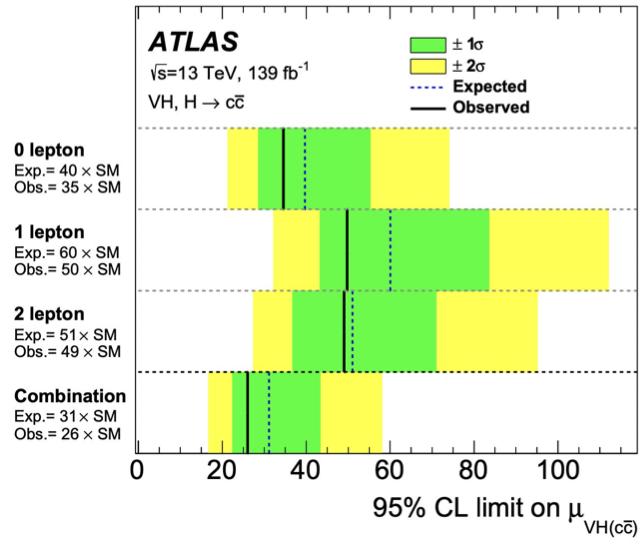
\includegraphics[width=\textwidth]{Images/VH/Fit/fromSlides/oldVHcc.%png}
    %    \caption{\vhc\ analysis \cite{Collaboration:2721696}.}
    %    \label{fig:fit_old_vhcclimit}
    %\end{subfigure}
    \begin{subfigure}[b]{0.48\textwidth}
        \centering
        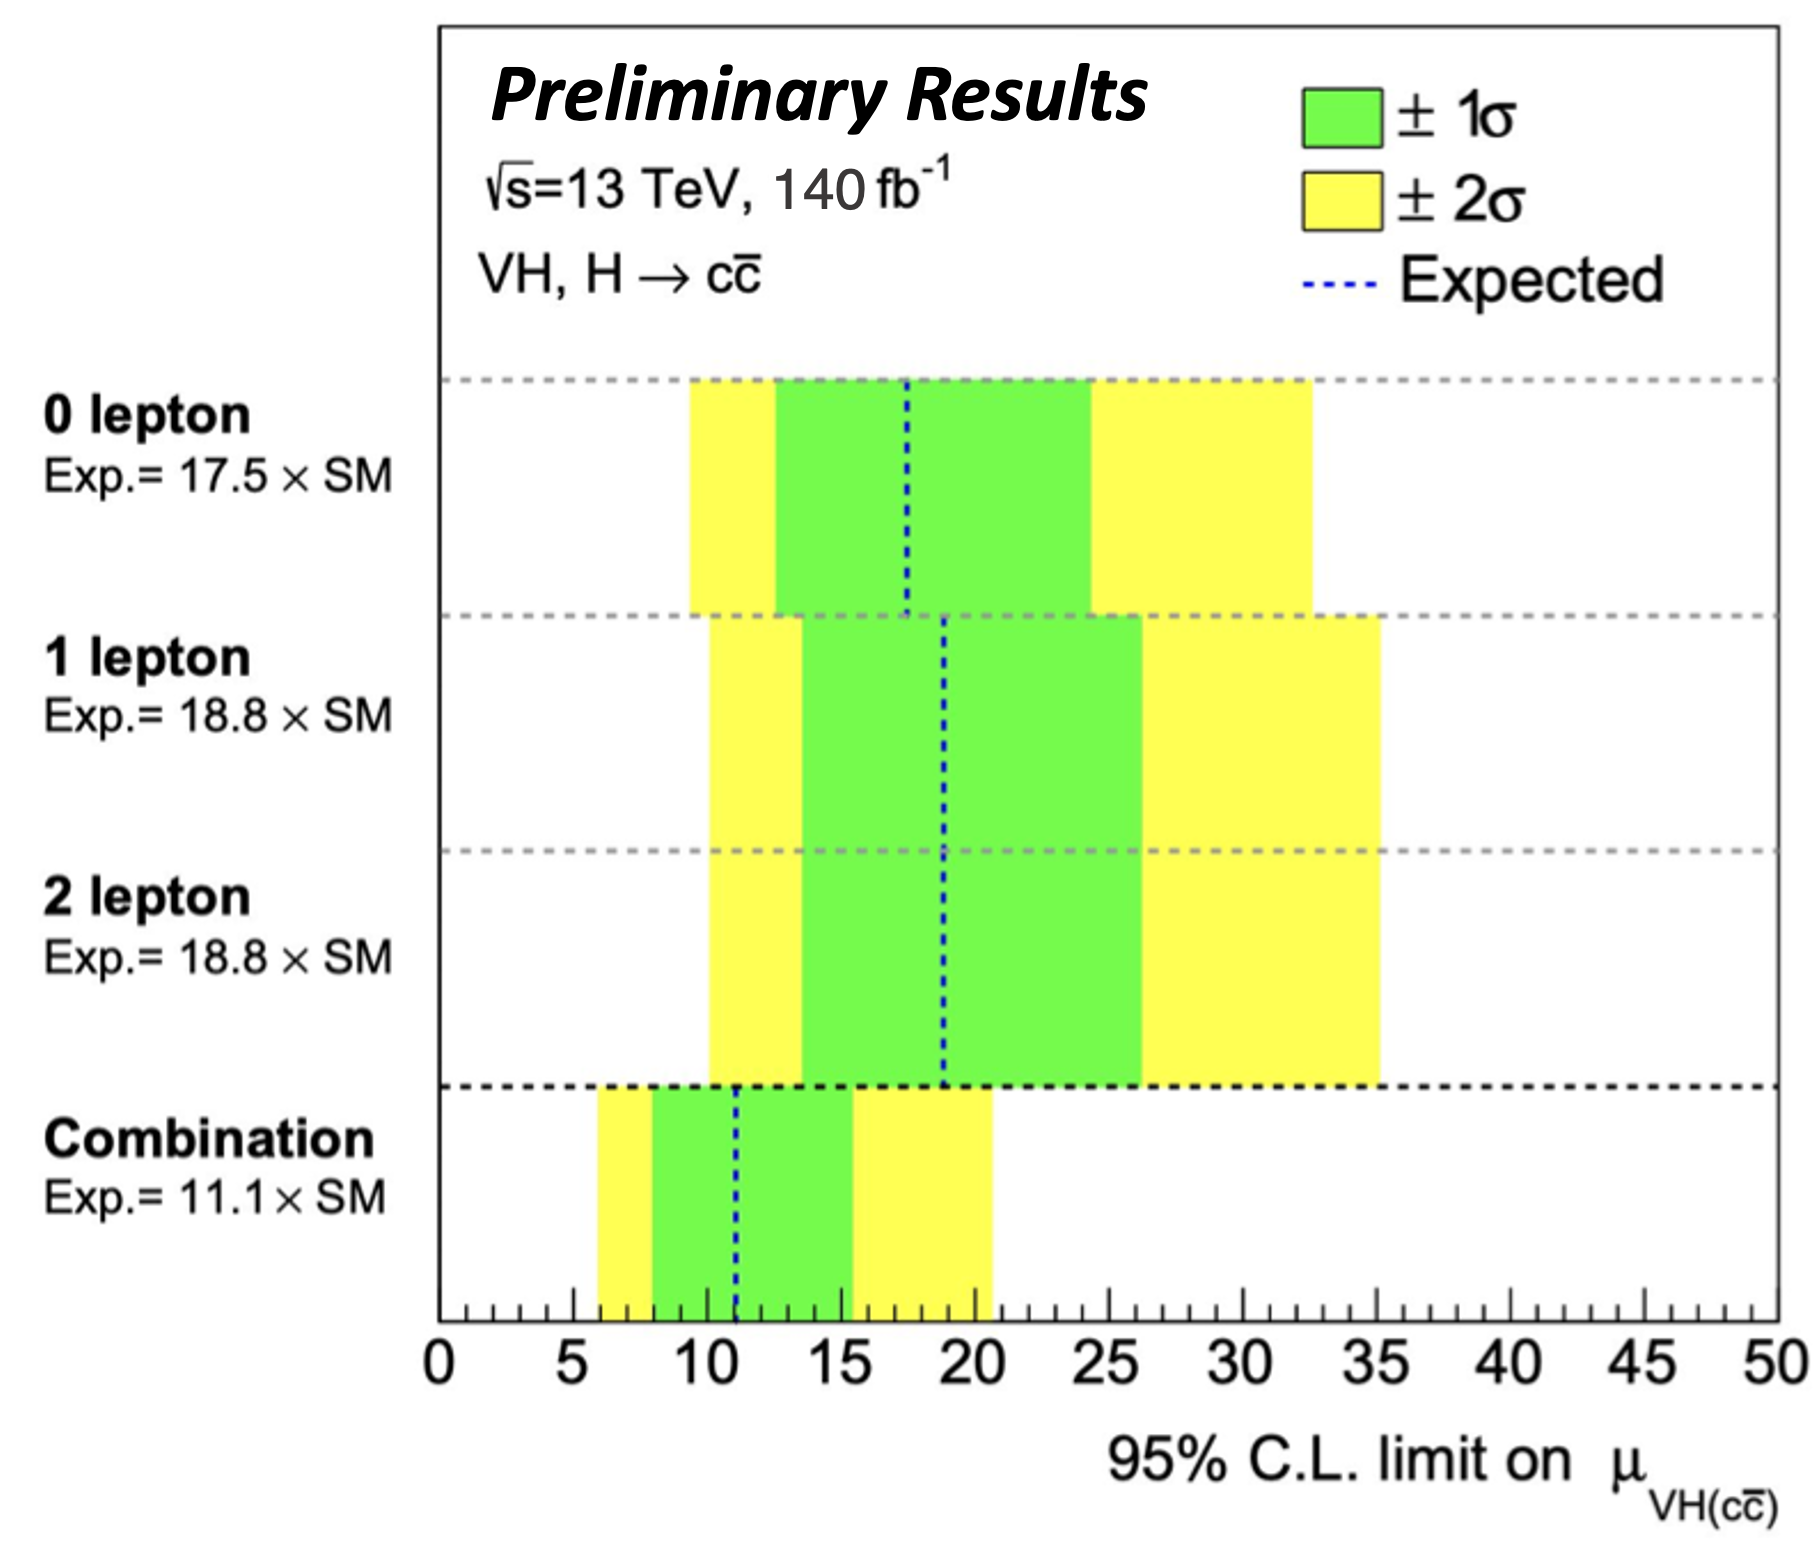
\includegraphics[width=\textwidth]{Images/VH/Fit/fromSlides/postfitVHcc.png}
        \caption{Postfit Asimov.}
        \label{fig:fit_new_vhcclimitPostfit}
    \end{subfigure}
    \begin{subfigure}[b]{0.48\textwidth}
      \centering
      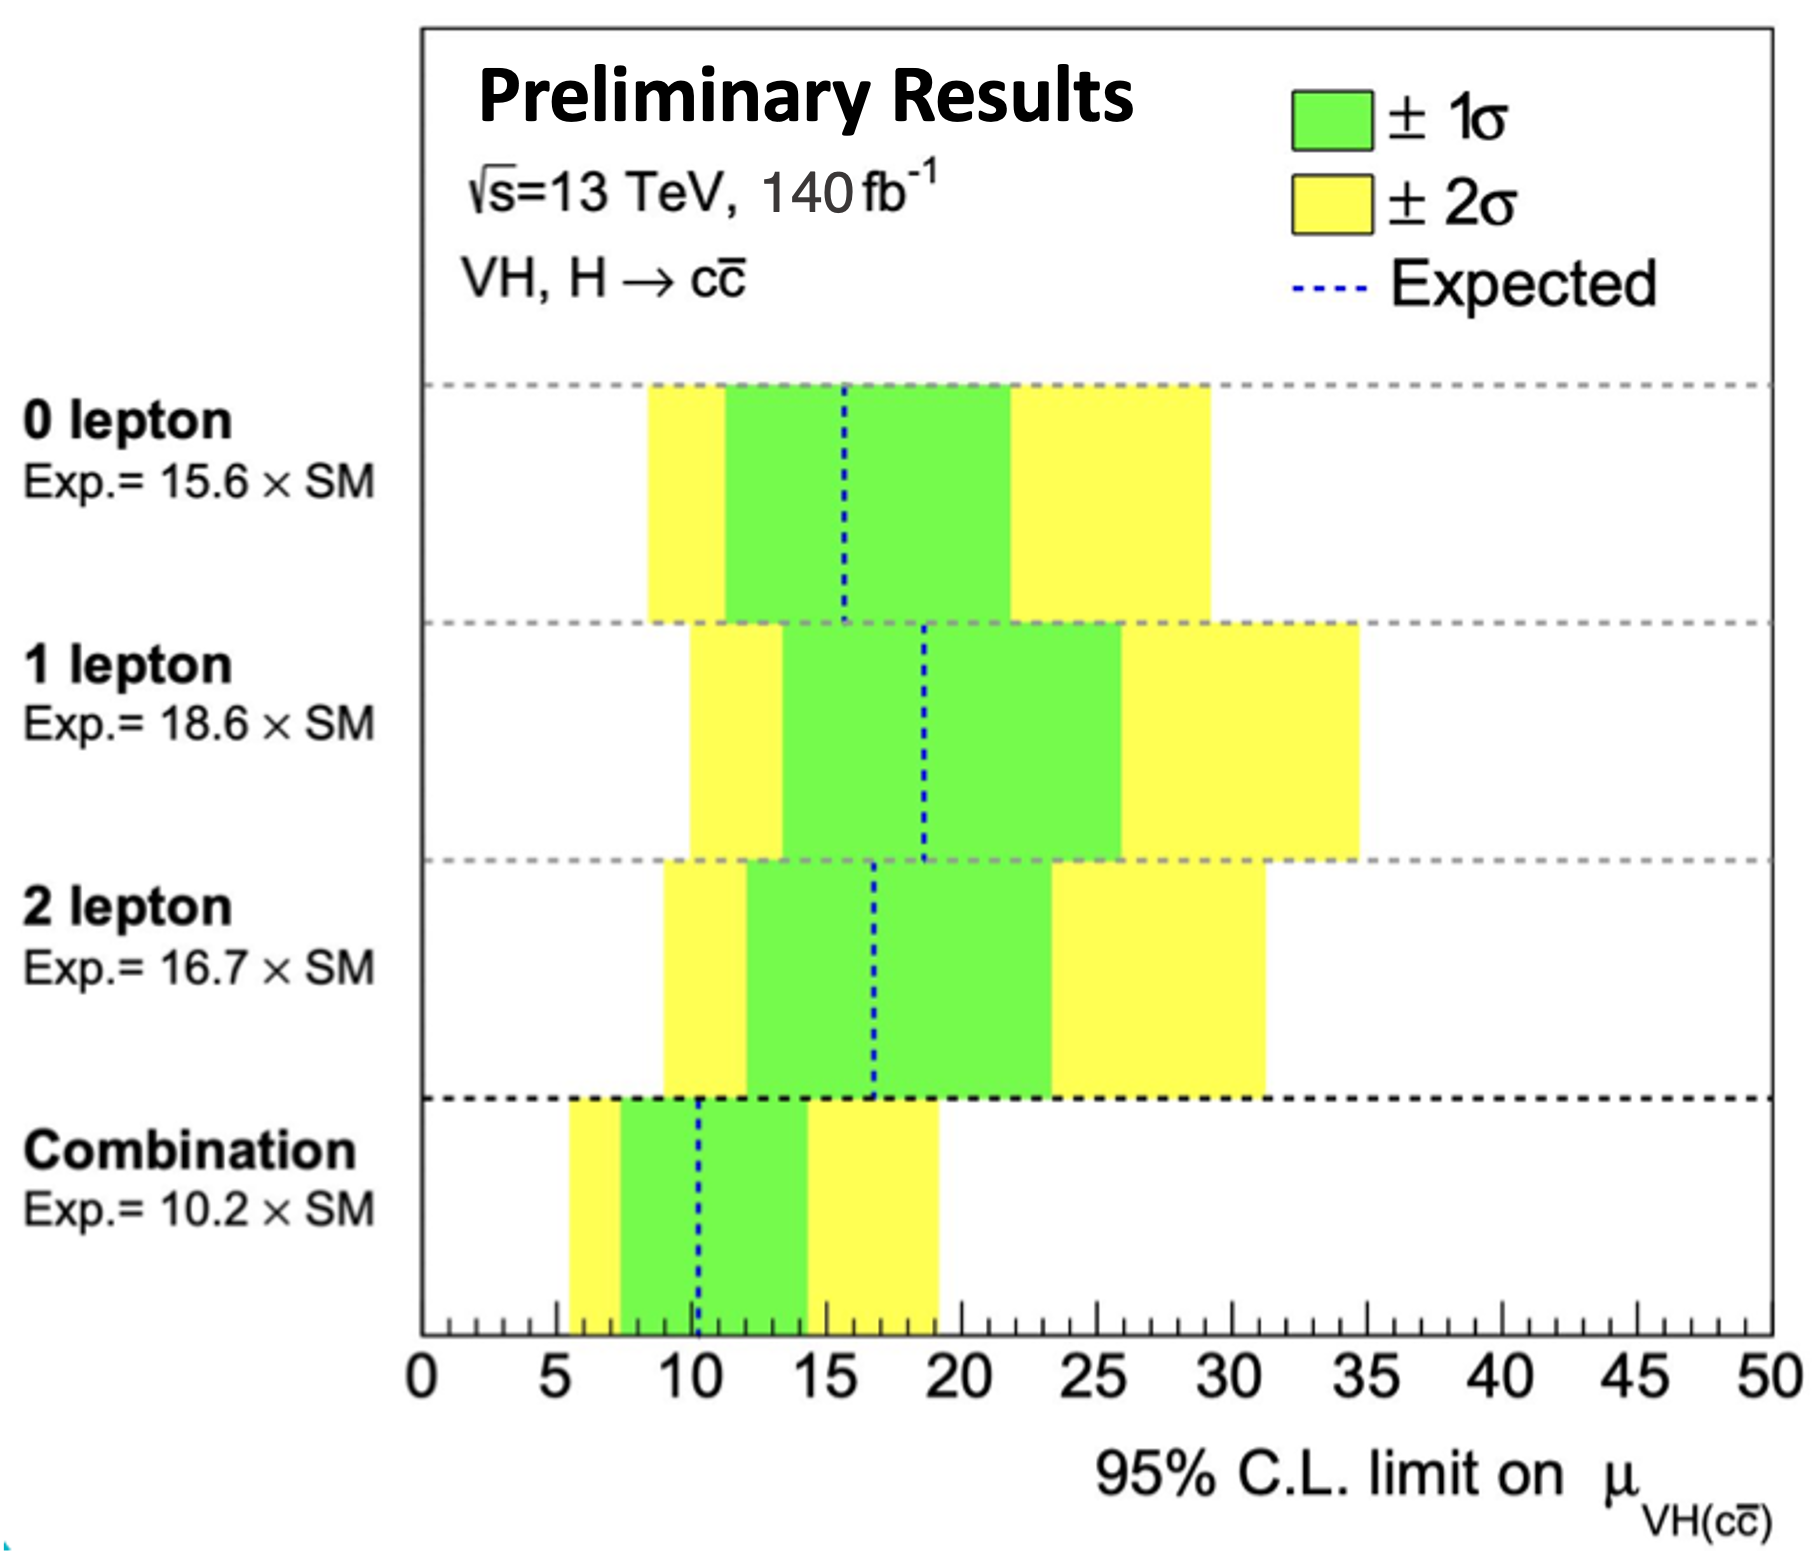
\includegraphics[width=\textwidth]{Images/VH/Fit/fromSlides/prefitVHcc.png}
      \caption{Prefit Asimov.}
      \label{fig:fit_new_vhcclimitPrefit}
  \end{subfigure}
    \caption{The 95\% CL$_s$ upper limit on the \vhc\ signal strength from the combined analysis postfit (left) and prefit (right) on the Asimov dataset.}
    \label{fig:fit_vhcc_limits}
\end{figure} 

Significant improvements are expected for all lepton channels. The combination of all lepton channels leads to a remarkable improvement on the 95\% \gls{cl}$_s$ upper limit on $\mu_{VHcc}$ from 31 $\times$ \gls{sm} in the latest ATLAS published \vhc\ result \cite{Collaboration:2721696}, to 11.1 $\times$ \gls{sm} (10.2 $\times$ \gls{sm}) in the postfit (prefit) Asimov fit of the combined analysis, a factor 2.8 improvements in sensitivity. Gains are expected to be made in all lepton channels, which now have similar sensitivity thanks to modifications to the analysis strategy. Compared to the published analysis, the 0-lepton channel upper limit is reduced from 40 $\times$ \gls{sm} $\rightarrow$ 17.5 $\times$ \gls{sm}, the 1-lepton from 60 $\times$ \gls{sm} $\rightarrow$ 18.8 $\times$ \gls{sm}, and the 2-lepton from 51 $\times$ \gls{sm} $\rightarrow$ 18.8 $\times$ \gls{sm} \cite{Collaboration:2721696}. These correspond to relative sensitivity improvement factors of 2.3, 3.2, and 2.7. Most of the gains are made in the 1- and 2-lepton channels, although the 0-lepton channel remains the most sensitive one.

%\subsubsection{\vhb}
\subsubsection{\boldvhb}
On the \vhb\ side, combining the resolved and boosted regime, the postfit expected significance on the \vhb\ signal strength is 7.9 $\sigma$ over the background-only prediction, corresponding to a 23\% improvement over the latest ATLAS published expected significance of 6.3 $\sigma$ \cite{ATLAS:2021wqh}. This is achieved thanks to a postfit expected significance of 4.7 $\sigma$ in the 0-lepton channel (15\% improvement to published result), 5.3 $\sigma$ in 1-lepton (30\% improvement), and 4.4 $\sigma$ in 2-lepton (3\% improvement). The most sensitive channel is now distinctively the 1-lepton channel. \\

Separating the \vhb\ signal strength into two \glspl{poi} for $WH(H \rightarrow{b\bar{b}})$ and $ZH(H \rightarrow{b\bar{b}})$, the prefit expected significances are 5.5 $\sigma$ for $WH$ and 6.2 $\sigma$ for $ZH$. This marks the first time a $H \rightarrow b\bar{b}$ analysis is expected to reach observation-level in $WH$, thanks to the large improvement in the 1-lepton channel sensitivity. \\

Finally, adopting the fine splitting of the \gls{stxs} stage 1.2 with 15 bins defined by \ptv\ and additional jet multiplicity \nj, with 8 bins in $ZH$ and 7 bins in $WH$, the \vhb\ analysis reaches the per bin sensitivities listed in Table \ref{tab:exp-stxs-prefit}, with evidence-level only attained for the $ZH$ 150 GeV < \ptv\ < 250 GeV without additional jet bin. The impact of systematics and statistical uncertainties on the signal strengths of the different bins is shown in Figure \ref{fig:fit-stxs-cons}. The measurement is particularly statistically limited. 

\begin{table}[h!]
    \centering
    \renewcommand*{\arraystretch}{1.2}
    \begin{tabular}{c r | C{4cm} C{4cm}}
        \hline \hline
        $VH$ & \multicolumn{1}{c|}{Truth \ptv} & 0 additional \nj & $\geq$1 additional \nj \\
        \hline
        WH &  [75, 150[ GeV & \multicolumn{2}{c}{0.69 $\sigma$} \\
        WH & [150, 250[ GeV & 2.29 $\sigma$ & 0.55 $\sigma$ \\
        WH & [250, 400[ GeV & 2.78 $\sigma$ & 0.94 $\sigma$ \\
        WH & [400, 600[ GeV & \multicolumn{2}{c}{1.87 $\sigma$} \\
        WH & $\geq$ 600 GeV & \multicolumn{2}{c}{1.43 $\sigma$} \\ \hline

        ZH &  [75, 150[ GeV & 1.48 $\sigma$ & 0.90 $\sigma$\\
        ZH & [150, 250[ GeV & 3.37 $\sigma$ & 1.64 $\sigma$ \\
        ZH & [250, 400[ GeV & 2.85 $\sigma$ & 1.49 $\sigma$ \\
        ZH & [400, 600[ GeV & \multicolumn{2}{c}{1.91 $\sigma$} \\
        ZH & $\geq$ 600 GeV & \multicolumn{2}{c}{1.07 $\sigma$} \\ 
        \hline \hline
    \end{tabular}
    \caption{The expected prefit significances in the different STXS bins of the combined analysis.}
    \label{tab:exp-stxs-prefit}
\end{table}

\begin{figure}[h!]
    \centering
    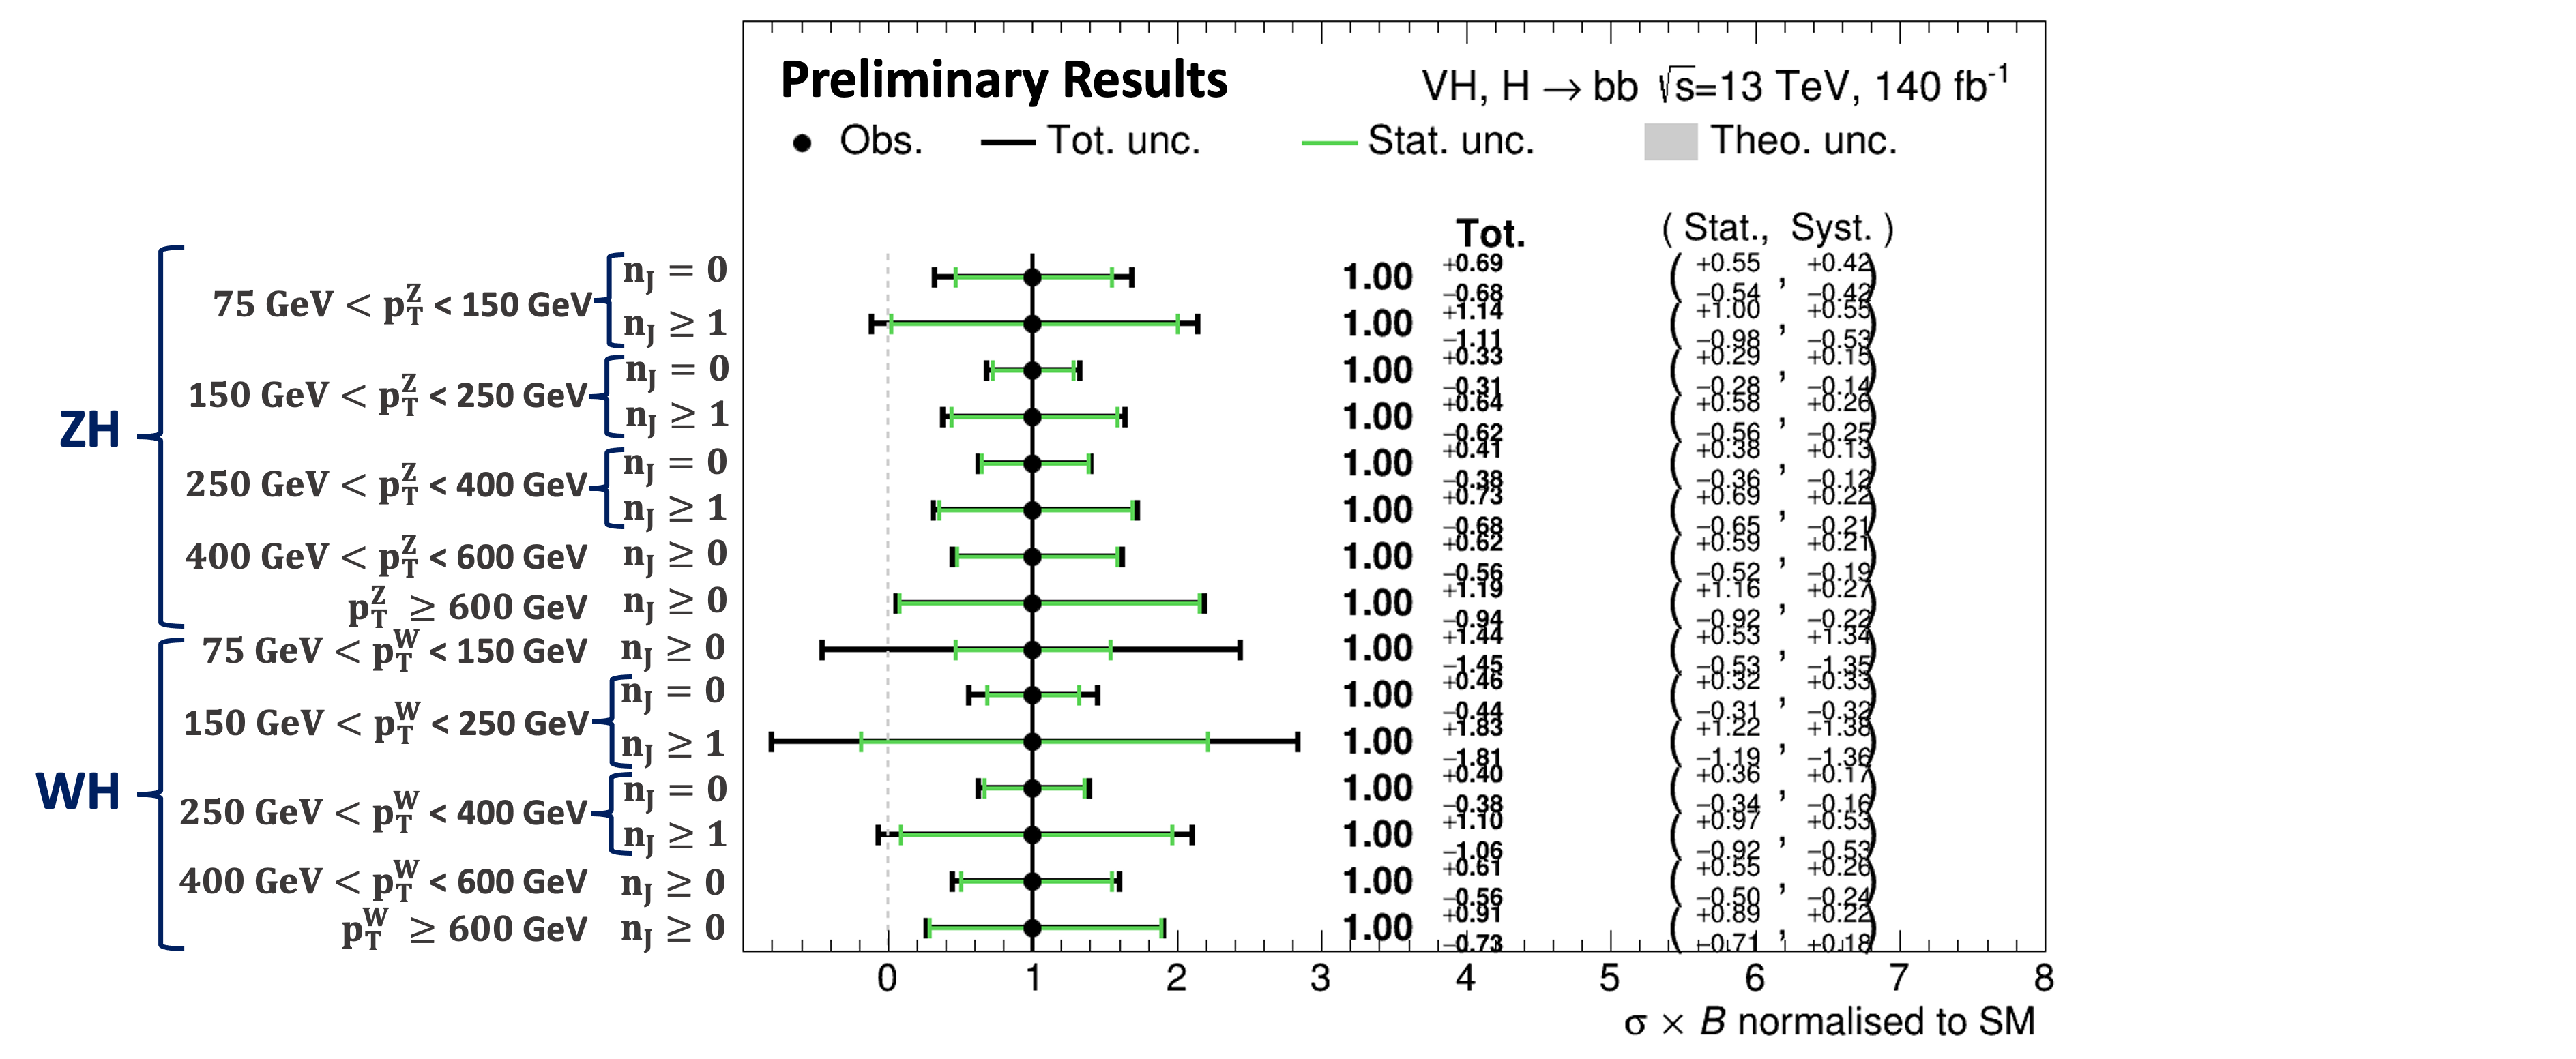
\includegraphics[width=\textwidth]{Images/VH/Fit/fromSlides/STXS_cons.png}
    \caption{The constraints on the prefit STXS signal strengths.}
    \label{fig:fit-stxs-cons}
\end{figure} 

\subsubsection{The Diboson Cross-Check}\label{subsec-DibosonC}
The diboson cross-check analysis is performed with the $VZ (\rightarrow b\bar{b})$ and $VZ (\rightarrow c\bar{c})$ as signals in a similar fashion to the \vhbc\ fit, to validate the strategy adopted. For the $VZ (\rightarrow b\bar{b})$ part, the postfit expected significance reaches a large value of 15.1 $\sigma$ when combining lepton channels. The 0-lepton, 1-lepton, and 2-lepton channels respectively reach postfit sensitivities of 11.2 $\sigma$, 6.2 $\sigma$, and 9 $\sigma$. On the $VZ (\rightarrow c\bar{c})$ side, the combined analysis expects to reach observation level for the first time, with a combined postfit expected significance of 5.1 $\sigma$. This represents a significant improvement of a factor 2.3 from the published 2.2 $\sigma$ expected result \cite{Collaboration:2721696}. The combined analysis reaches a postfit expected significance of 3.9 $\sigma$ in 0-lepton, 2.6 $\sigma$ in 1-lepton, and 3.1 $\sigma$ in 2-lepton.

\subsubsection{Additional Fit Results}
In addition to the main results highlighted above, some further insights into the output of the fits are given before concluding this chapter. To verify that the Monte Carlo samples correctly model the data after the fit, some postfit plots are presented in Figure \ref{fig:postfit_SR_CR} for selected signal and control regions. All the postfit analysis distributions are listed in Appendix \ref{appsec-vh-analRegPosfit}. Interestingly, good agreement between the data and postfit \gls{mc} samples is also observed in validation regions not directly constrained in the fit. Figure \ref{fig:postfitval} displays postfit distributions for a $BL$-tagged region analoguous to the included $BT$-tagged Top CR, an $LL$-tagged region similar to the $c$-tagged signal region, and the \ptv\ spectrum of the inclusive 2L $BB$-tagged 2-jet signal region. The good agreement observed between data and \gls{mc}-samples in all regions is evidence of a sufficient fit constraining. \\


\begin{figure}[h!]
    \centering
    \begin{subfigure}[b]{0.32\textwidth}
        \centering
        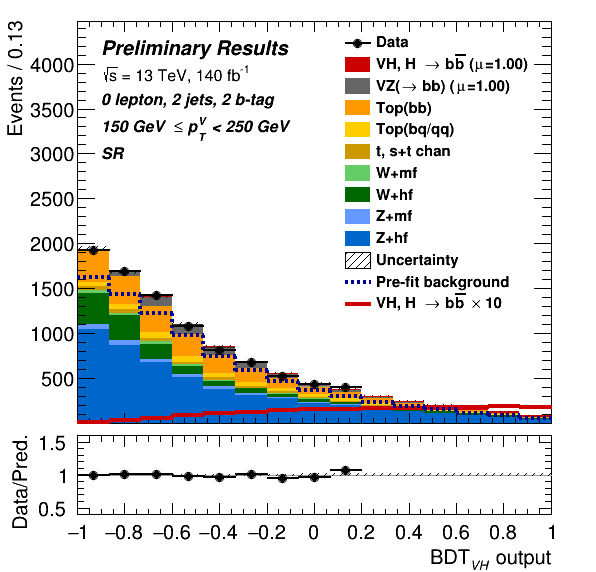
\includegraphics[width=\textwidth]{Images/VH/Own_fit/postfit_VHbb/Region_distmva_BMax250_BMin150_DSR_J2_TTypebb_T2_L0_Y6051_GlobalFit_conditionnal_mu1.png}
        \caption{0L, 2-jet 150 GeV $<$ \ptv\ $<$ 250 GeV $BB$-tagged.}
        \label{fig:posfit_0L_SR}
    \end{subfigure}
    \begin{subfigure}[b]{0.32\textwidth}
        \centering
        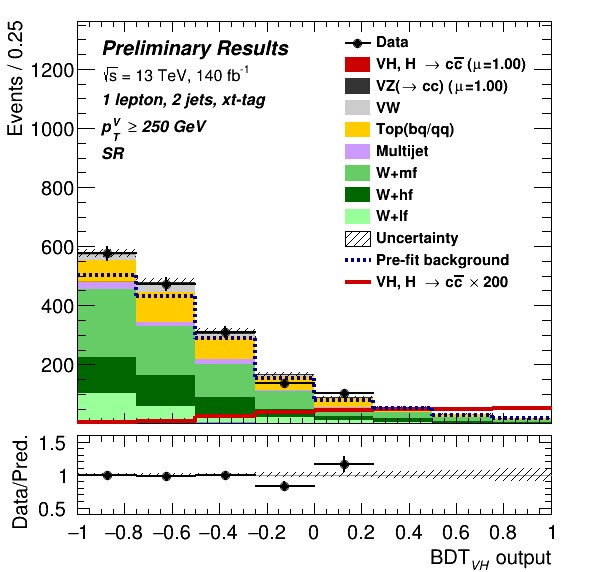
\includegraphics[width=\textwidth]{Images/VH/Own_fit/postfit_VHcc/Region_distmva_BMin250_DSR_J2_TTypext_T2_L1_Y6051_GlobalFit_conditionnal_mu1.png}
        \caption{1L, 2-jet \ptv\ $>$ 250 GeV 2 $c$-tagged.}
        \label{fig:posfit_1L_SR}
    \end{subfigure}
    \begin{subfigure}[b]{0.32\textwidth}
      \centering
      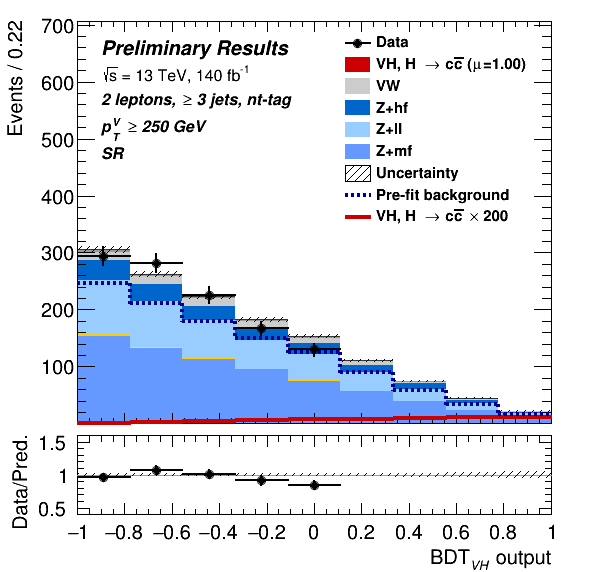
\includegraphics[width=\textwidth]{Images/VH/Own_fit/postfit_VHcc/Region_distmva_BMin250_DSR_J3_TTypent_incJet1_T1_L2_Y6051_GlobalFit_conditionnal_mu1.png}
      \caption{2L, $\geq$3-jet \ptv\ $>$ 250 GeV 1 $c$-tagged.}
      \label{fig:posfit_2L_SR}
    \end{subfigure} \\
    \begin{subfigure}[b]{0.32\textwidth}
        \centering
        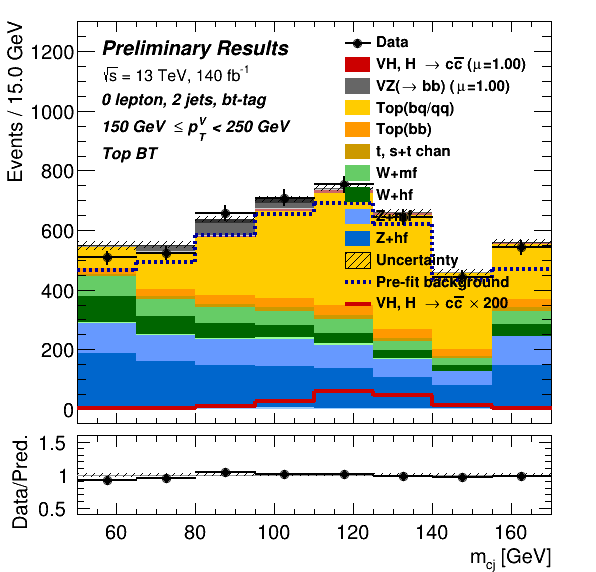
\includegraphics[width=\textwidth]{Images/VH/Own_fit/postfit_VHcc/Region_distmBB_BMax250_BMin150_DtopCRBC_J2_TTypebt_T1_L0_Y6051_GlobalFit_conditionnal_mu1.png}
        \caption{0L, 2-jet 150 GeV $<$ \ptv\ $<$ 250 GeV Top $BT$ CR.}
        \label{fig:posfit_0L_CR}
    \end{subfigure}
    \begin{subfigure}[b]{0.32\textwidth}
        \centering
        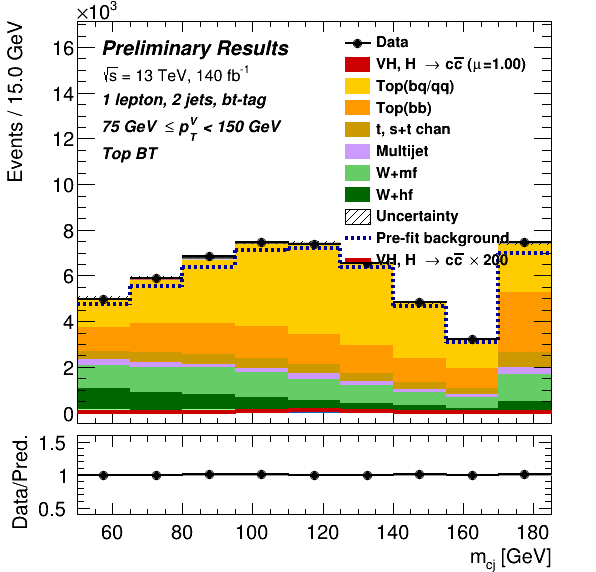
\includegraphics[width=\textwidth]{Images/VH/Own_fit/postfit_VHcc/Region_distmBB_BMax150_BMin75_DtopCRBC_J2_TTypebt_T1_L1_Y6051_GlobalFit_conditionnal_mu1.png}
        \caption{1L, 2-jet 75 GeV $<$ \ptv\ $<$ 150 GeV Top $BT$ CR.}
        \label{fig:posfit_1L_CR}
    \end{subfigure}
    \begin{subfigure}[b]{0.32\textwidth}
        \centering
        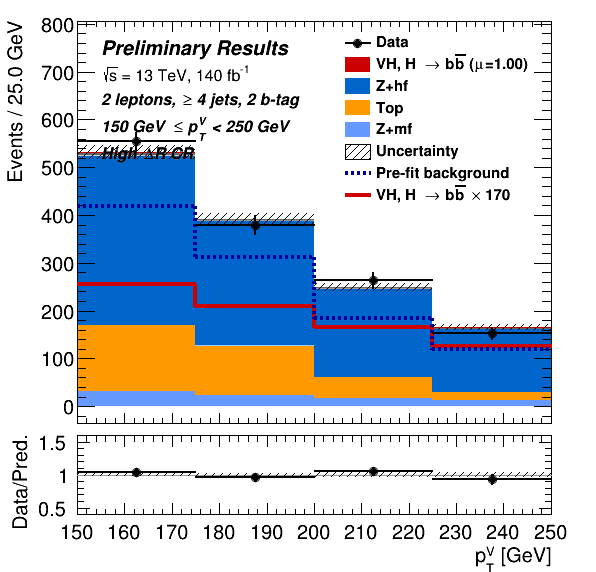
\includegraphics[width=\textwidth]{Images/VH/Own_fit/postfit_VHbb/Region_distpTV_BMax250_BMin150_DCRHigh_J4_TTypebb_incJet1_T2_L2_Y6051_GlobalFit_conditionnal_mu1.png}
        \caption{2L, $\geq$ 4-jet 250 GeV $<$ \ptv\ $<$ 400 GeV $BB$-tagged CRHigh.}
        \label{fig:posfit_2L_CR}
    \end{subfigure}
    \caption{Selected postfit signal regions (top row) and control regions (bottom row), for the 0L (left), 1L (centre), and 2L (right).}
    \label{fig:postfit_SR_CR}
\end{figure} 

\begin{figure}[h!]
    \centering
    \begin{subfigure}[b]{0.32\textwidth}
        \centering
        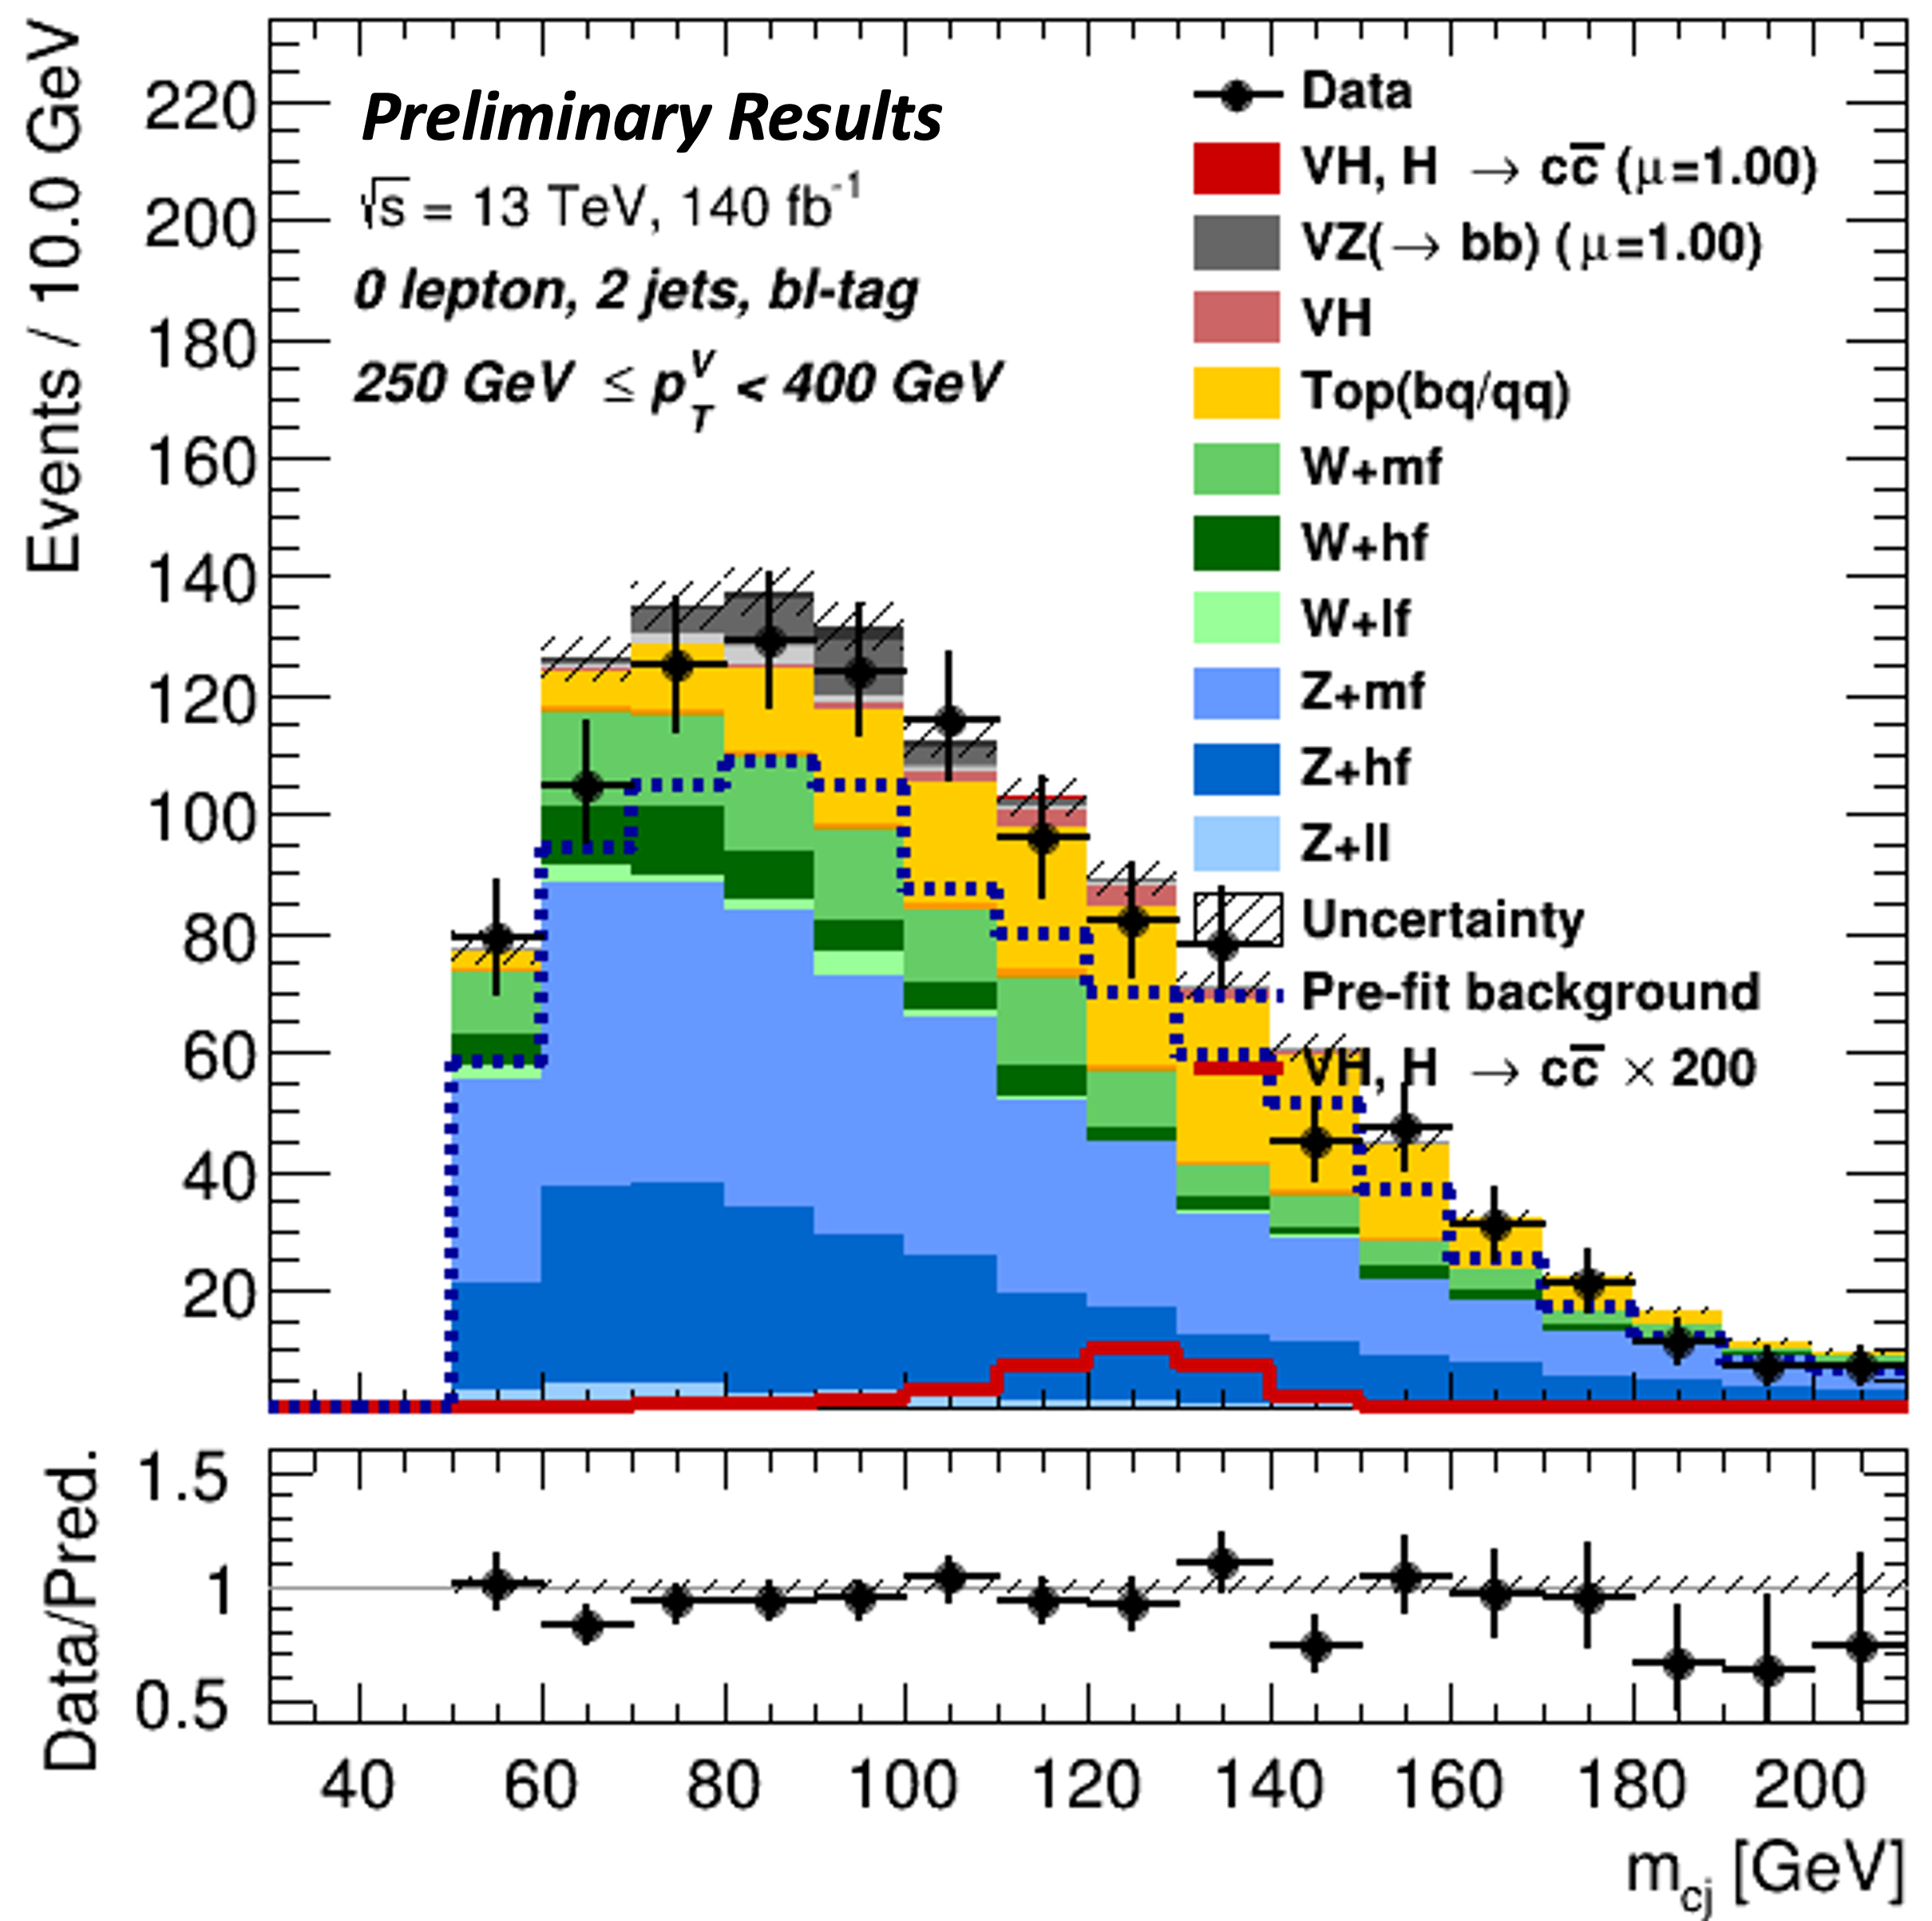
\includegraphics[width=\textwidth]{Images/VH/Fit/fromSlides/Postfit/0LtopCRBL.png}
        \caption{0L $BL$-tagged, TopCR-like.}
        \label{fig:val_BLtopCR}
    \end{subfigure}
    \begin{subfigure}[b]{0.32\textwidth}
        \centering
        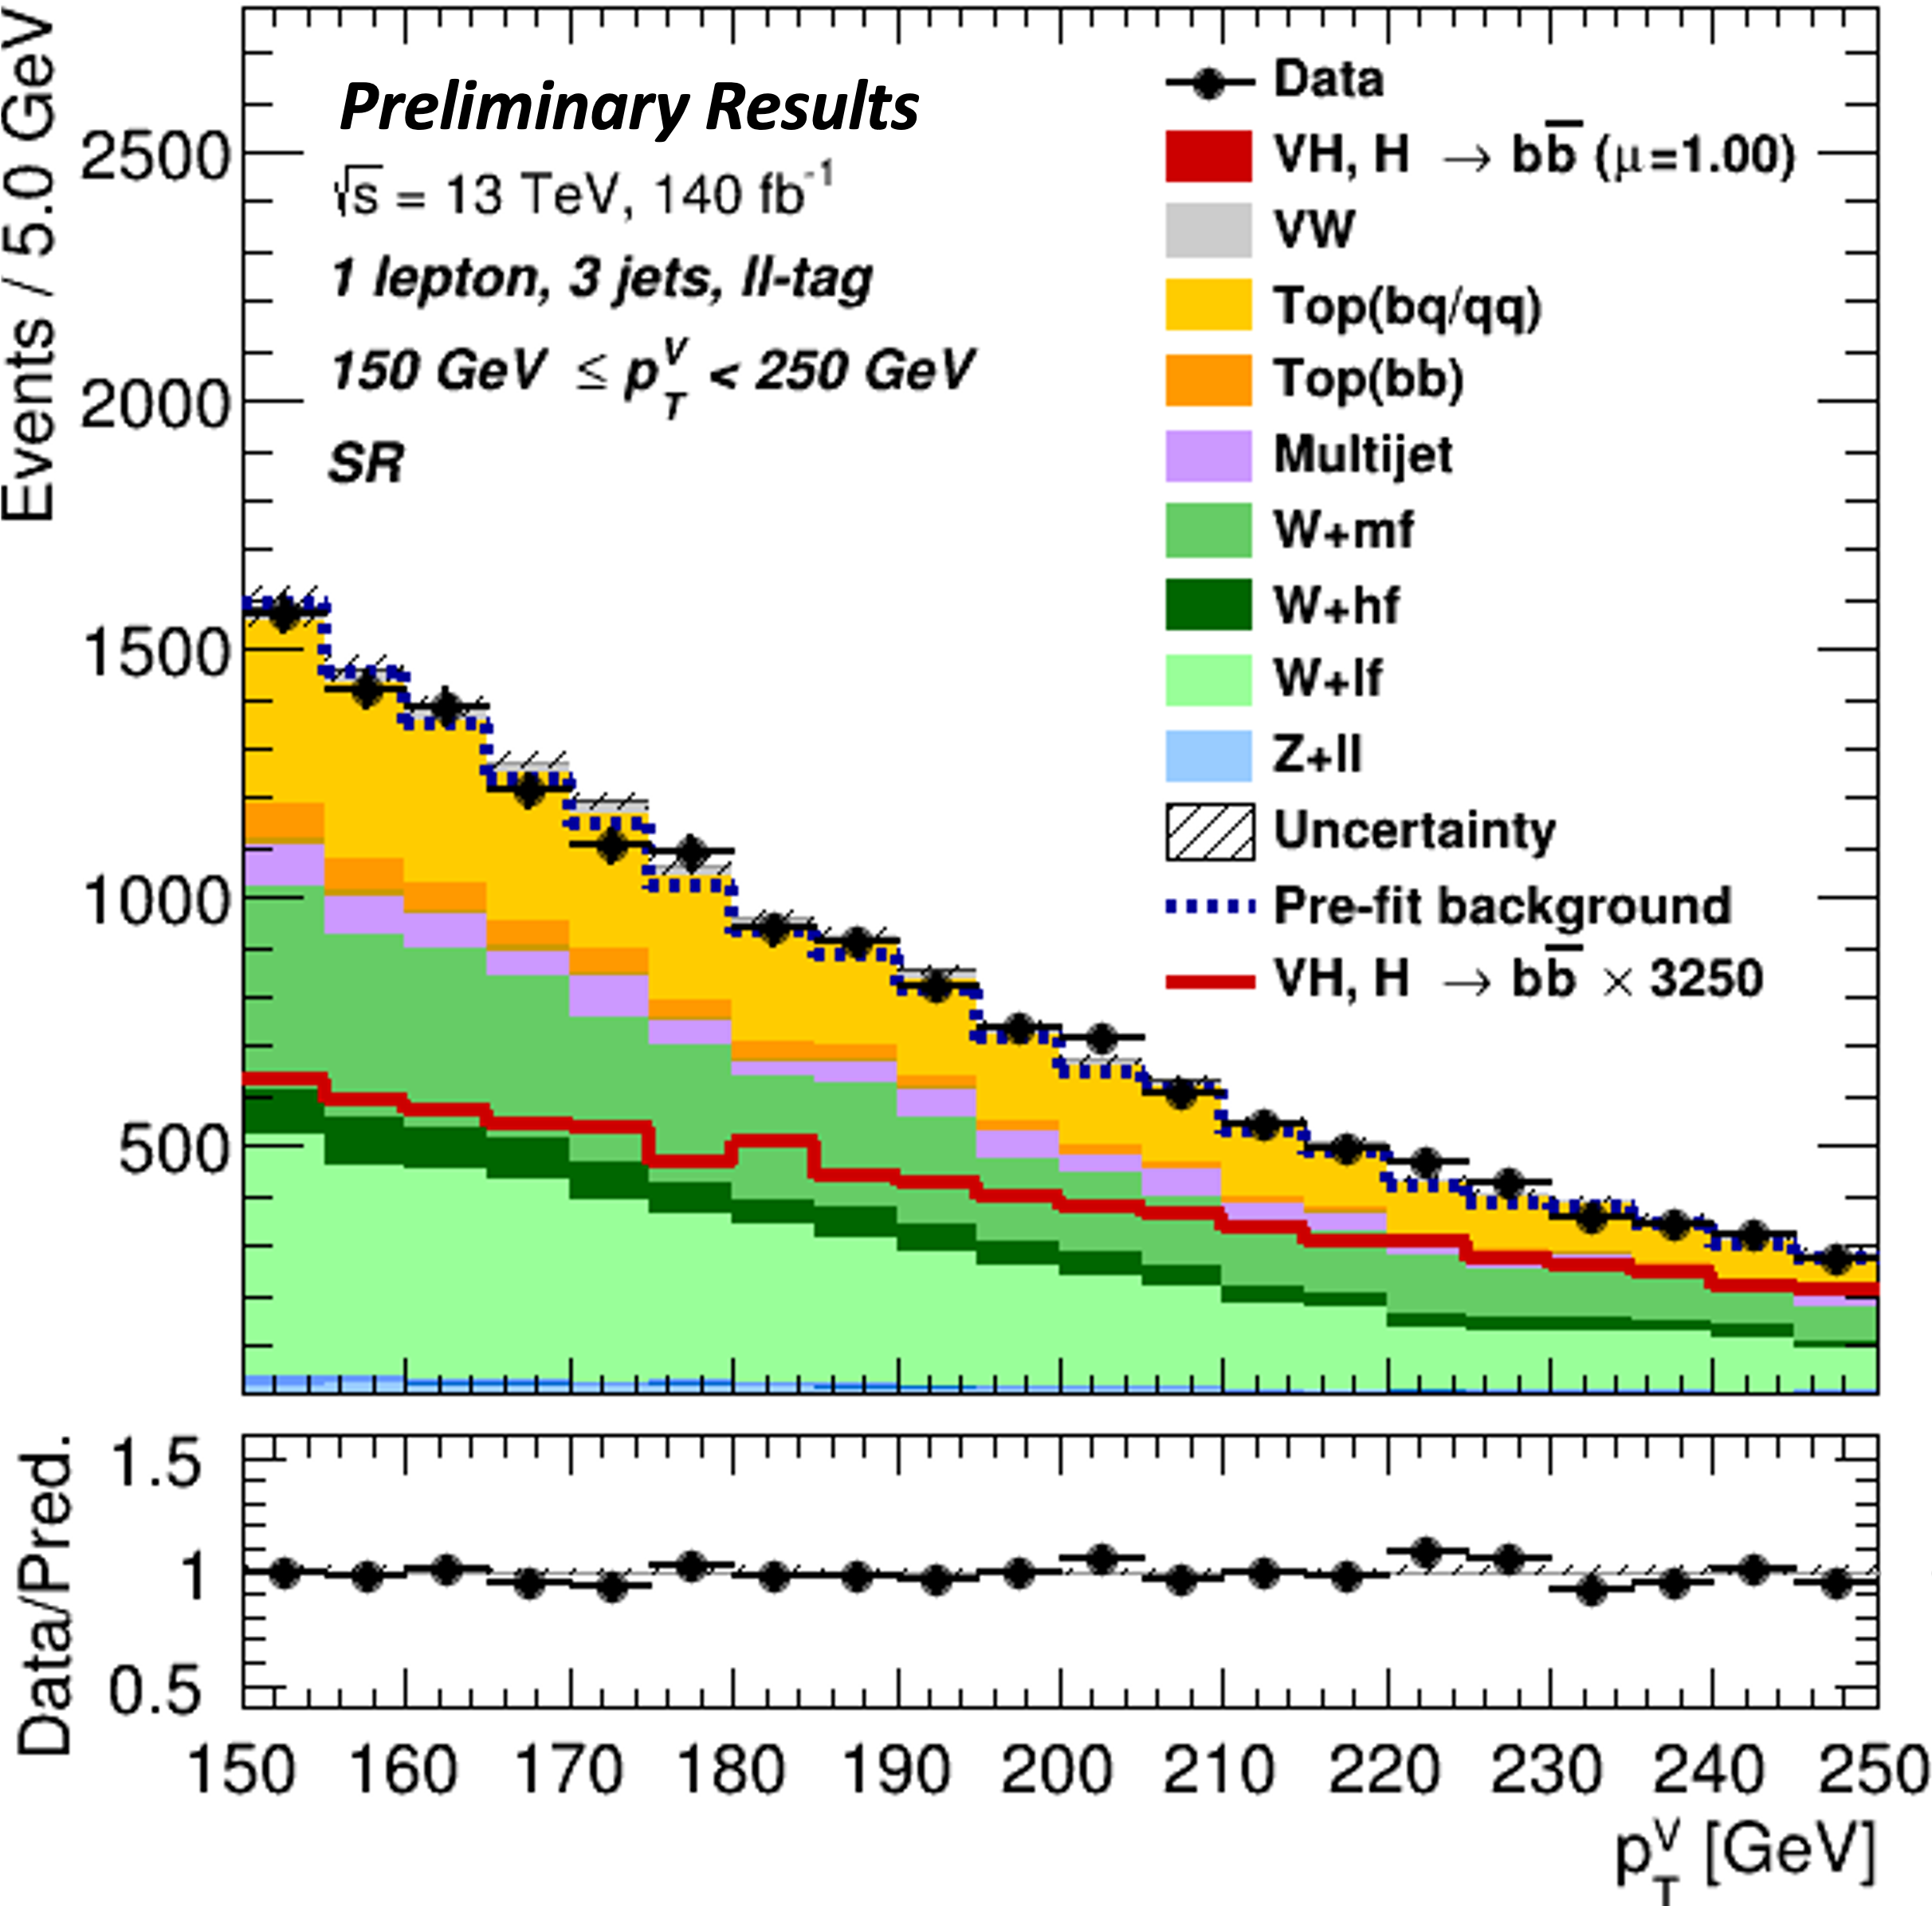
\includegraphics[width=\textwidth]{Images/VH/Fit/fromSlides/Postfit/1L_LLSR.png}
        \caption{1L $LL$, $c$-tagged SR-like.}
        \label{fig:val_LLSR}
    \end{subfigure}
    \begin{subfigure}[b]{0.32\textwidth}
      \centering
      \includegraphics[width=\textwidth]{Images/VH/Fit/fromSlides/Postfit/2LBB.png}
      \caption{2L \ptv\ in 2-jets $BB$ SR.}
      \label{fig:fit_ptv2L}
    \end{subfigure} 
    \caption{Posfit distributions in a $BL$-tagged Top CR-like (left) and $LL$-tagged SR-like (centre) validations regions and the 2L \ptv\ spectrum in the 2-jet $BB$-tagged SR.}
    \label{fig:postfitval}
\end{figure} 

The breakdown of the uncertainties, presented in Table \ref{tab:exp-breakdown}, is a measure of the different contributions of the uncertainties to the \vhbc\ analysis. The \glspl{np} are grouped based on their origin, and their impact on the signal strengths of \vhb\ and \vhc\ is assessed by iteratively re-running fits with successive groups of \glspl{np} fixed at their postfit values. The notation adopted is to label the signal strengths of the nominal maximal likelihood fit as $\hat{\mu}$ with uncertainty $\hat{\sigma_{\mu}}$, and of a re-run fit with a group of \glspl{np} fixed at $\hat{\mu}'$ with uncertainty $\sigma_{\hat{\mu}'}$. The impact of the fixed group of \glspl{np} is defined as the change in uncertainty measured by 

\begin{table}[h!]
    \centering
    \renewcommand*{\arraystretch}{1.3}
    \begin{tabular}{l  C{2cm} C{2cm}}
        \hline \hline
        Source of Uncertainty & $\mu_{VH(H\rightarrow b\bar{b})}$ & $\mu_{VH(H\rightarrow c\bar{c})}$ \\
        \hline
        \textbf{Total}               &  0.127 & 5.089 \\
        \textbf{Statistics}          &  0.095 & 3.791 \\
        \textbf{Systematics }        &  0.085 & 3.395 \\ 
        \hline \hline
        \textbf{Statistical Uncertainties} & 0.095 & 3.791 \\
        Data sample size             &  0.088 & 3.538 \\
        Floating normalisations      &  0.029 & 1.247 \\
        Top $e\mu$ CR statistics     &  0.011 & 0.130 \\ 
        \hline \hline
        \textbf{Systematics Uncertainties} & 0.085 & 3.395 \\ 
        \vhbc\ Modelling         & 0.021 & 0.237 \\
        \hline
        \textbf{Backgrounds Modelling}    & 0.069 & 2.739 \\
        $Z+$jets                     &  0.036 & 1.587 \\
        $W+$jets                     &  0.036 & 1.088 \\
        Diboson                      &  0.020 & 0.546 \\
        \ttb\                        &  0.011 & 0.613 \\
        single-top                   &  0.008 & 0.116 \\
        Multi-jet                    &  0.007 & 0.691 \\
        \hline
        \textbf{Experimental Uncertainties} & 0.035 & 1.278 \\
        Jet                          &  0.026 & 0.737 \\
        Large-$R$ jet                &  0.009 & 0.206 \\
        \etm\                        &  0.007 & 0.150 \\
        Lepton                       &  0.004 & 0.115 \\
        FTAG PFlow ($b$-jet)         &  0.015 & 0.258 \\
        FTAG PFlow ($c$-jet)         &  0.008 & 0.769 \\
        FTAG PFlow (light-jet)         &  0.003 & 0.751 \\
        FTAG PFlow (extrap)          &  0.000 & 0.000 \\
        FTAG VR ($b$-jet)            &  0.004 & 0.049 \\
        FTAG VR ($c$-jet)            &  0.001 & 0.018 \\
        FTAG VR (light-jet)            &  0.001 & 0.009 \\
        FTAG VR (extrap)             &  0.001 & 0.037 \\
        Pile-up                      &  0.005 & 0.052 \\
        Luminosity                   &  0.007 & 0.035 \\
        \hline
        \textbf{MC-samples Size}     &  0.020 & 1.410 \\
        \hline \hline
    \end{tabular}
    \caption{Breakdown of the different systematics and statistical uncertainties.}
    \label{tab:exp-breakdown}
\end{table}

\begin{equation}
    \text{Impact} = \sqrt{\hat{\sigma_{\mu}}^2 - \hat{\sigma_{\mu}'}^2}.
\end{equation}
To evaluate the impact of the statistical uncertainties, a fit is run with all \glspl{np} fixed except for the floating normalisations. The total systematics effect is set to the difference in quadrature between the total and the statistical uncertainties. For both the \vhb\ and \vhc\ measurements, the statistical and systematic uncertainties are of similar size, with the statistical uncertainties being slightly larger. The uncertainties are far smaller for the \vhb\ side, as expected from the larger statistics and better performance of both the experimental reconstruction and modelling. For \vhb, the largest contributions to the systematics uncertainties come from the $V+$jets and diboson background modelling, and the signal modelling. The importance of the $V+$jets is expected since the $W+$jets and $Z+$jets play a significant role in the 1-lepton and the 0- and 2-lepton channels respectively. On the experimental side, the jet and flavour tagging uncertainties are leading. For the latter, the $b$-jets uncertainties contribute the most followed by the $c$-jets, as expected from the resemblance between heavy-flavour jet species. \\

For \vhc, similar observations are made with several nuances. On the modelling side, the signal modelling is less paramount, with the top and multi-jet processes contributing more significantly. Additionally, the $Z+$jets uncertainties are now clearly leading, with the $W+$jets proportionally less important. This latter observation is connected with the larger importance of the top processes, as \vhc\ has a much larger top contribution in the 1-lepton channel, competing with $W+$jets as the leading source of uncertainty there. On the experimental side, the flavour tagging uncertainties of the $c$- and light-jets are now dominant, with the jet reconstruction uncertainties. This is expected from the challenges of tagging and reconstructing $c$-jets. The statistic of the \gls{mc}-samples is far more important on the \vhc\ side, mostly due to the low $c$-tagging efficiency of the \gls{dl1r} tagger used. \\

A second technique to assess the importance of different nuisance parameters on the signal strengths is to change their \gls{np} values upwards and downwards by their postfit uncertainties $\sigma_{\theta}$ and re-run the fit with the modified \gls{np} fixed. For each \gls{np}, this requires running two fits in addition to the nominal fit from which $\hat{\theta}$ and $\hat{\sigma_{\theta}}$ are measured: one with the \gls{np} fixed at $\hat{\theta} + \hat{\sigma_{\theta}}$ and one with $\hat{\theta} - \hat{\sigma_{\theta}}$. \glspl{np} are ranked by the difference in the signal strengths between these new fits and the nominal one, as shown in Figure \ref{fig:rankingPostfit}. In these plots, the central values of \glspl{np} are set at 0 (at 1 for \glspl{fn} and $\gamma$-factor) as the dataset is the postfit Asimov set. \\

For \vhb, the \whf\ extrapolations have a significant impact on the predicted signal strength, with several of those systematics highly ranked. Shape uncertainties associated with the diboson process and Higgs modelling uncertainties as well as the $Wt$ DS-DR shape uncertainty and $b$-jet tagging uncertainties also contribute meaningfully. The floating normalisation of \whf\ in the boosted region is the only \gls{fn} to make the ranking, due to its significant pull, as is shown in Figure \ref{fig:FNback}. \\

For \vhc, the Top process \gls{carl} shapes are the leading nuisance parameters, with the $Z+cc$ shape and the $W+$jets $cc/bb$ acceptance ratio. The \zlf\ and, to a lesser extent, the \wlf\ floating normalisations have a large impact on the predicted signal strength, despite the constraints offered by the $V+l$ \gls{cr}. The light- and $c$-jets uncertainties from flavour tagging are the biggest contributors in this category. Finally, the multi-jet normalisation enters the ranking as this process contributes more in \vhc. The $\gamma$-factor listed corresponds to the last unblinded bin in the 1L high \ptv\ 2-jet \gls{sr} shown in Figure \ref{fig:posfit_1L_SR}, where a large amount of signal is expected, and the effect of this \gls{np} should be reduced once the signal is no longer constrained to its \gls{sm} expectations in the final unblinded conditional fit to data.

\begin{figure}[h!]
    \centering
    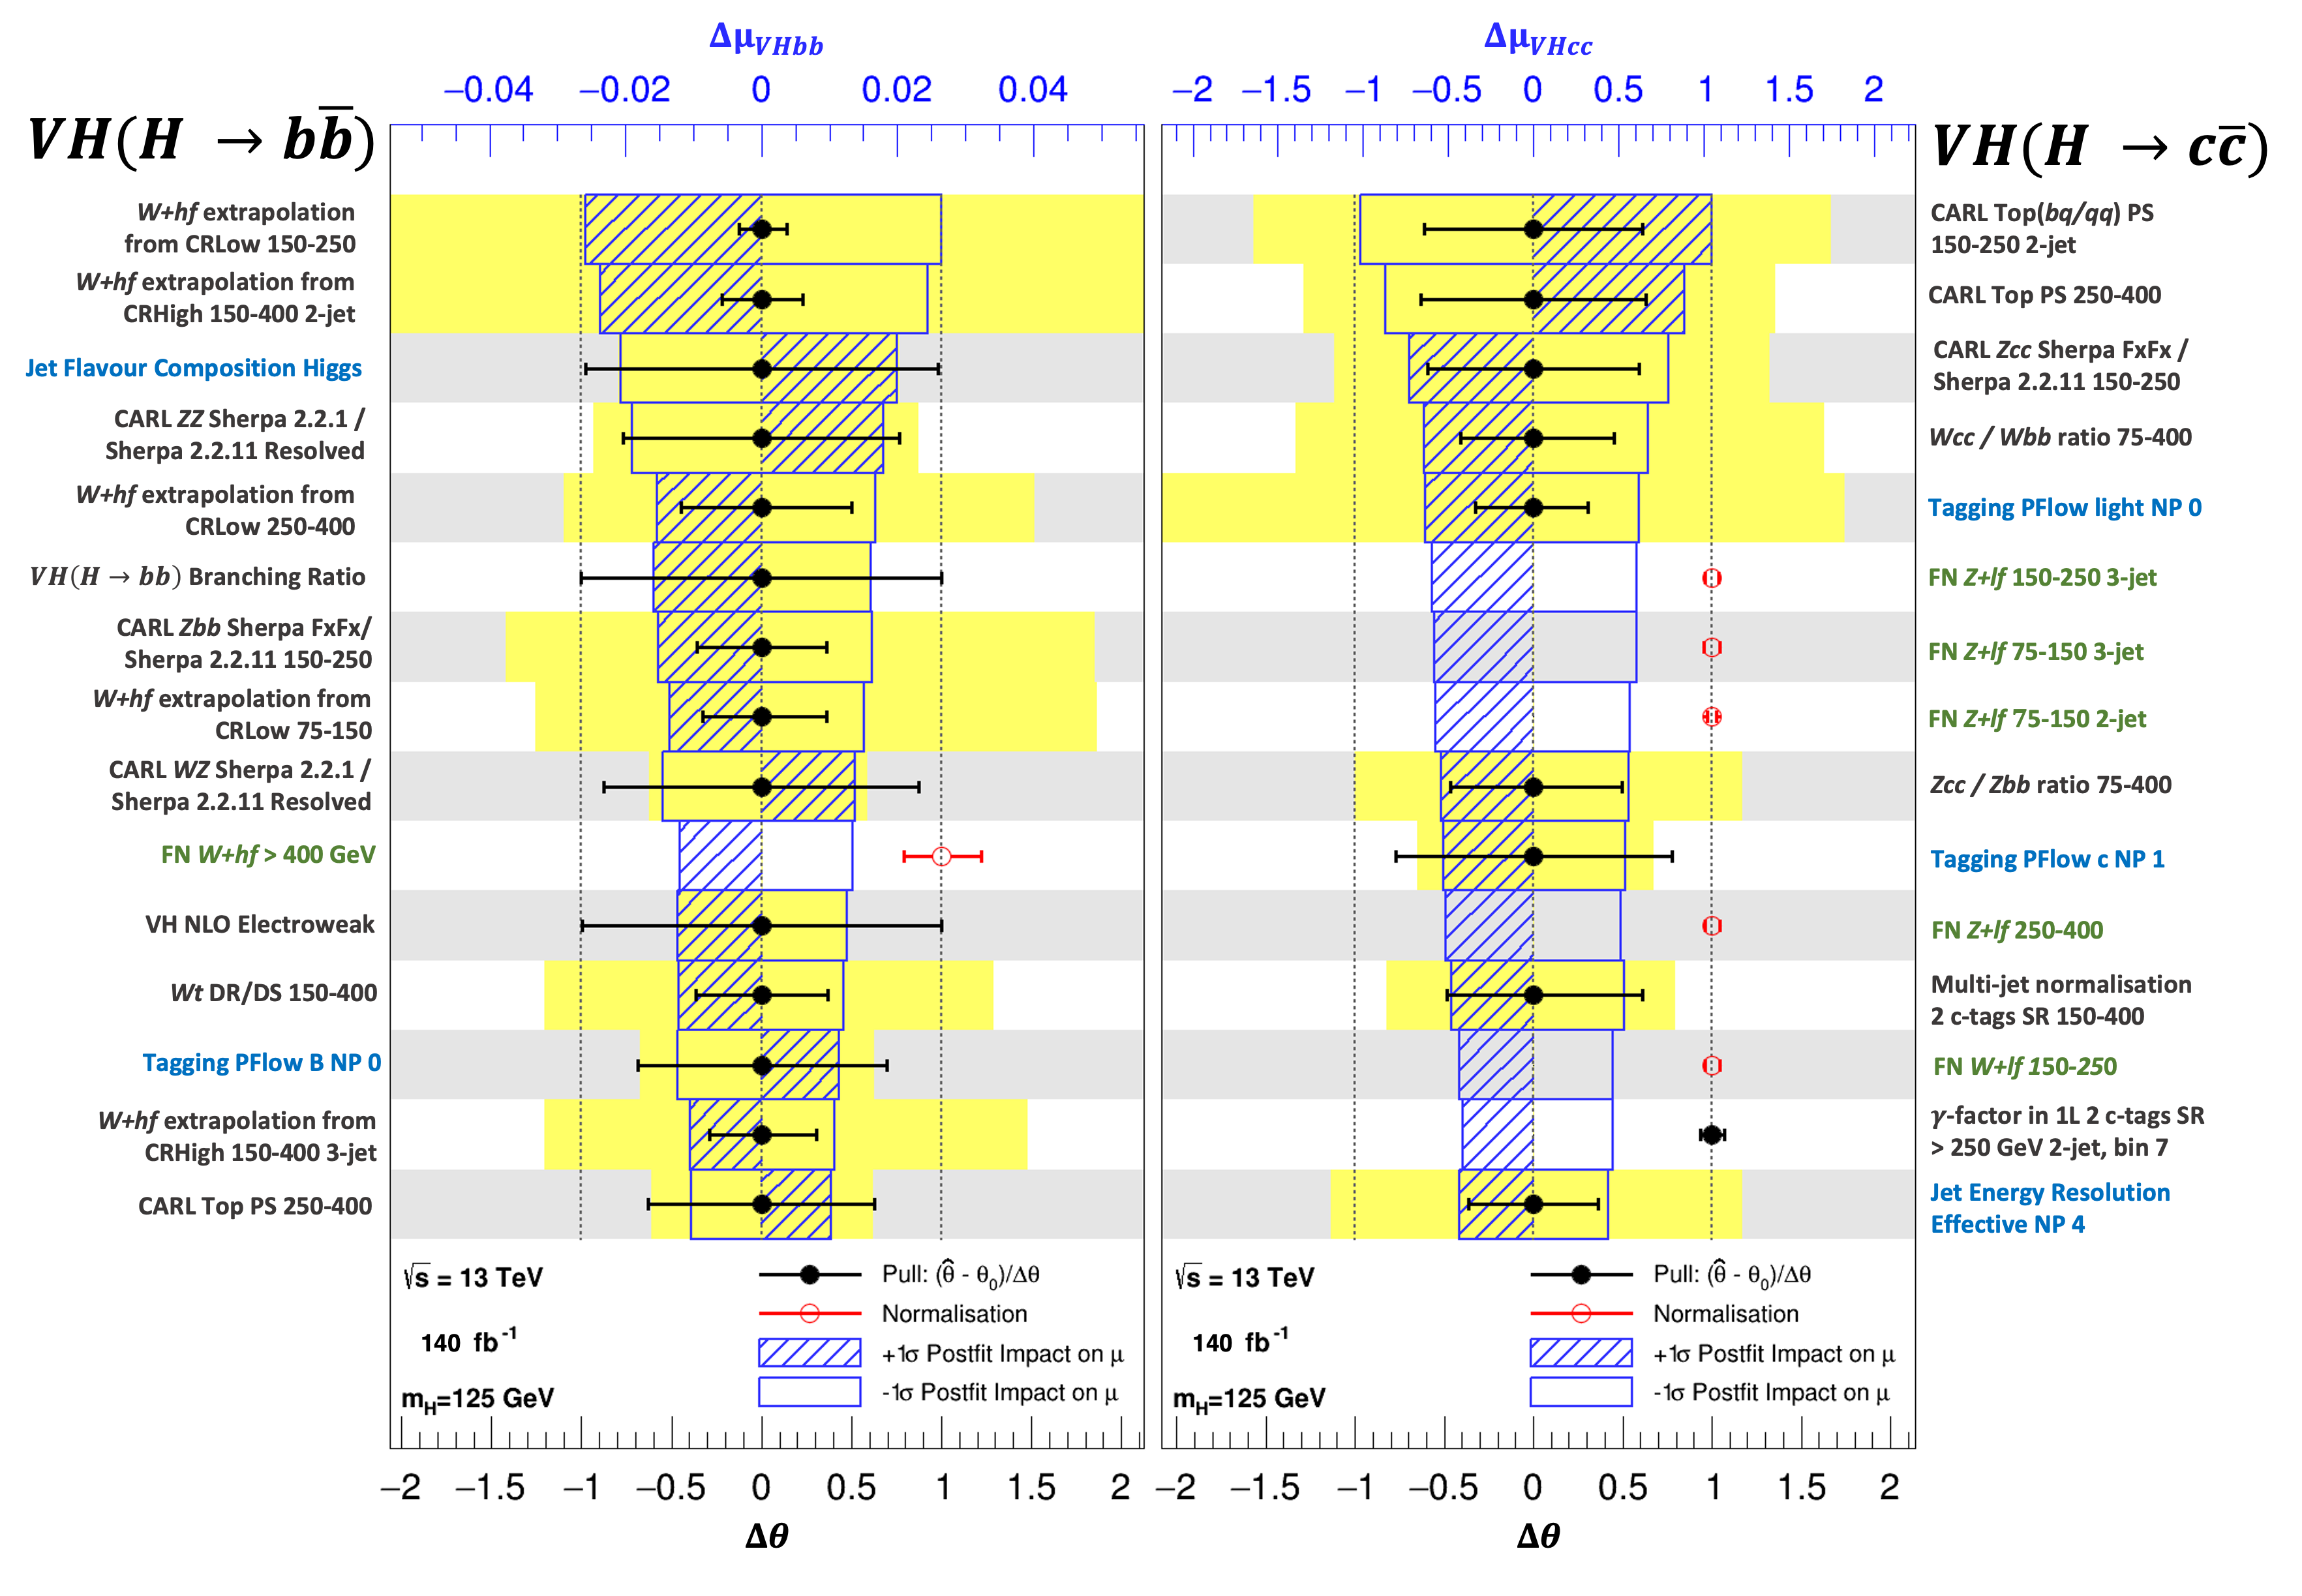
\includegraphics[width=\textwidth]{Images/VH/Fit/fromSlides/ranking.png}
    \caption{The 15 most highly ranked Asimov postfit nuisance parameters for the \vhb\ (left) and \vhc\ (right) signal strengths. Modelling NPs are written in black, experimental NPs in blue, and floating normalisation (and $\gamma$-factor) in green, with values indicated by the bottom axis showing $\Delta \theta = \hat{\theta} - \theta_0$. Black points are nuisance parameters with their central value at 0 showing the pull ($\gamma$-factor with central value at 1), and red points are floating normalisation with central values at 1. The error bars on the point show the 1 $\sigma$ uncertainty of the NP. The effect of changing the NP by +1 $\sigma$ (-1 $\sigma$) induces the change in signal strength $\Delta\mu$ shown by the hashed (empty) blue rectangle, defined with respect to the top axis.}
    \label{fig:rankingPostfit}
\end{figure} 

\begin{figure}[h!]
    \centering
    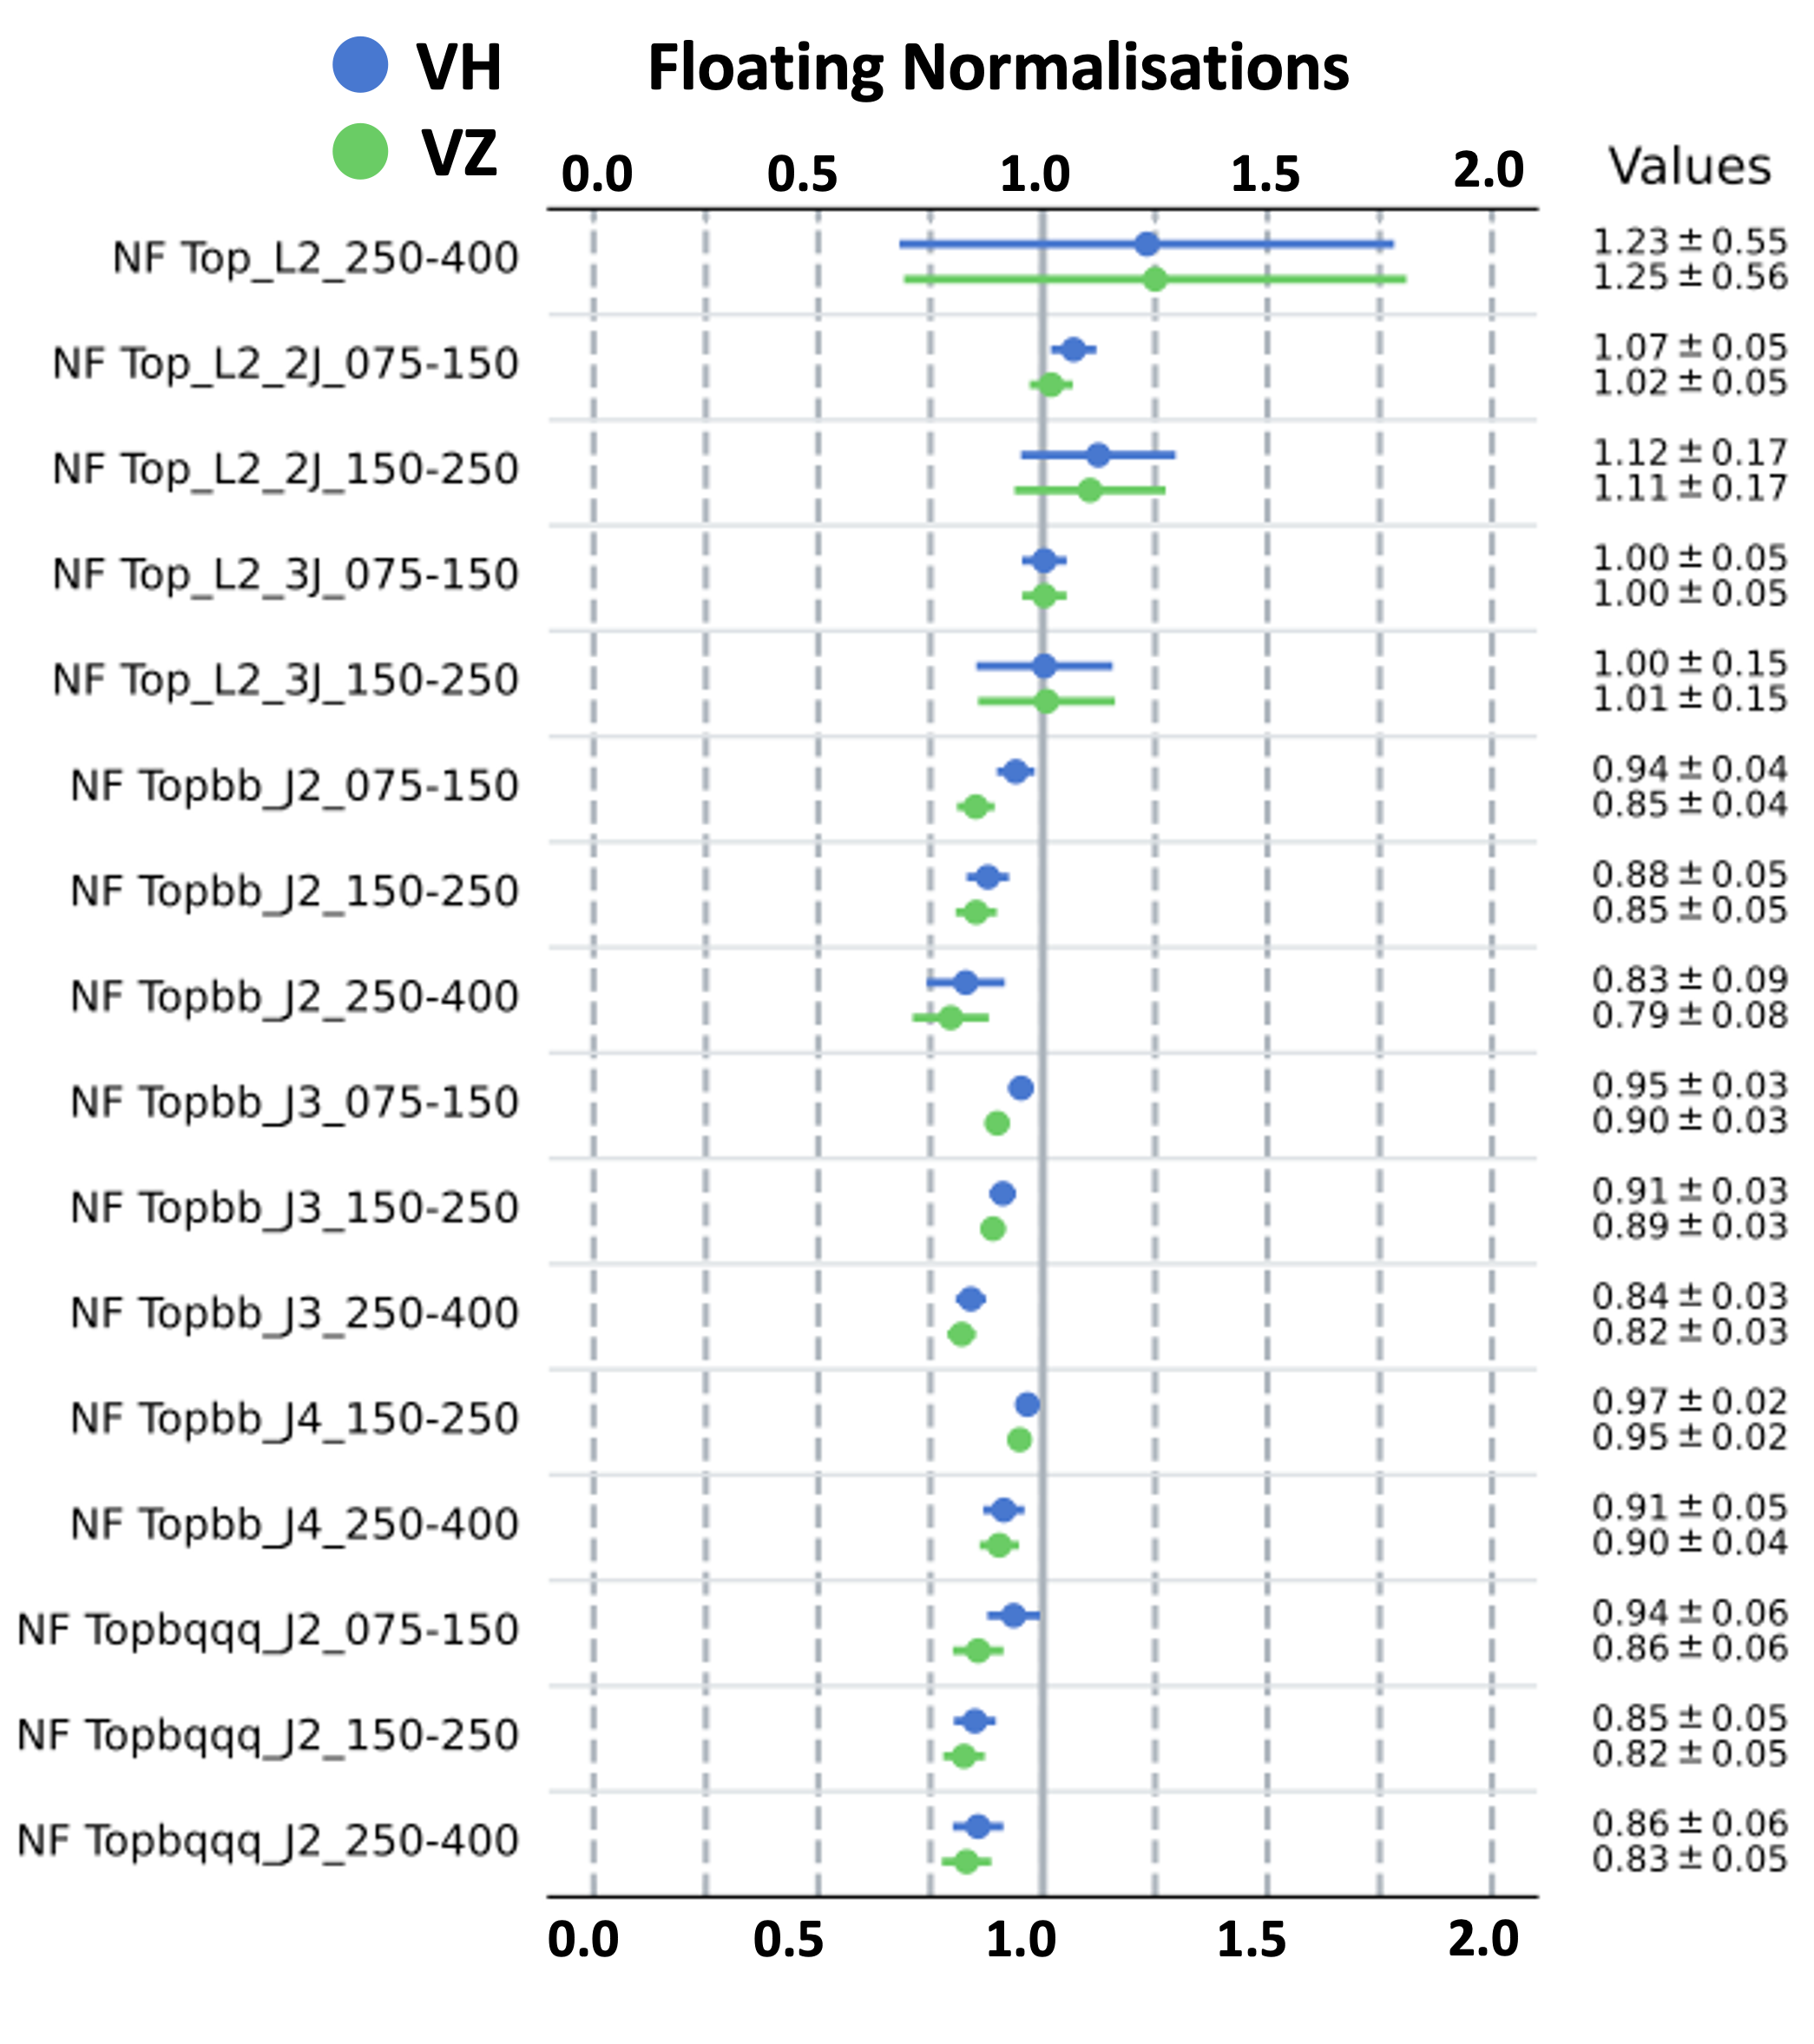
\includegraphics[width=0.49\textwidth]{Images/VH/Fit/fromSlides/FN/FN1.png}
    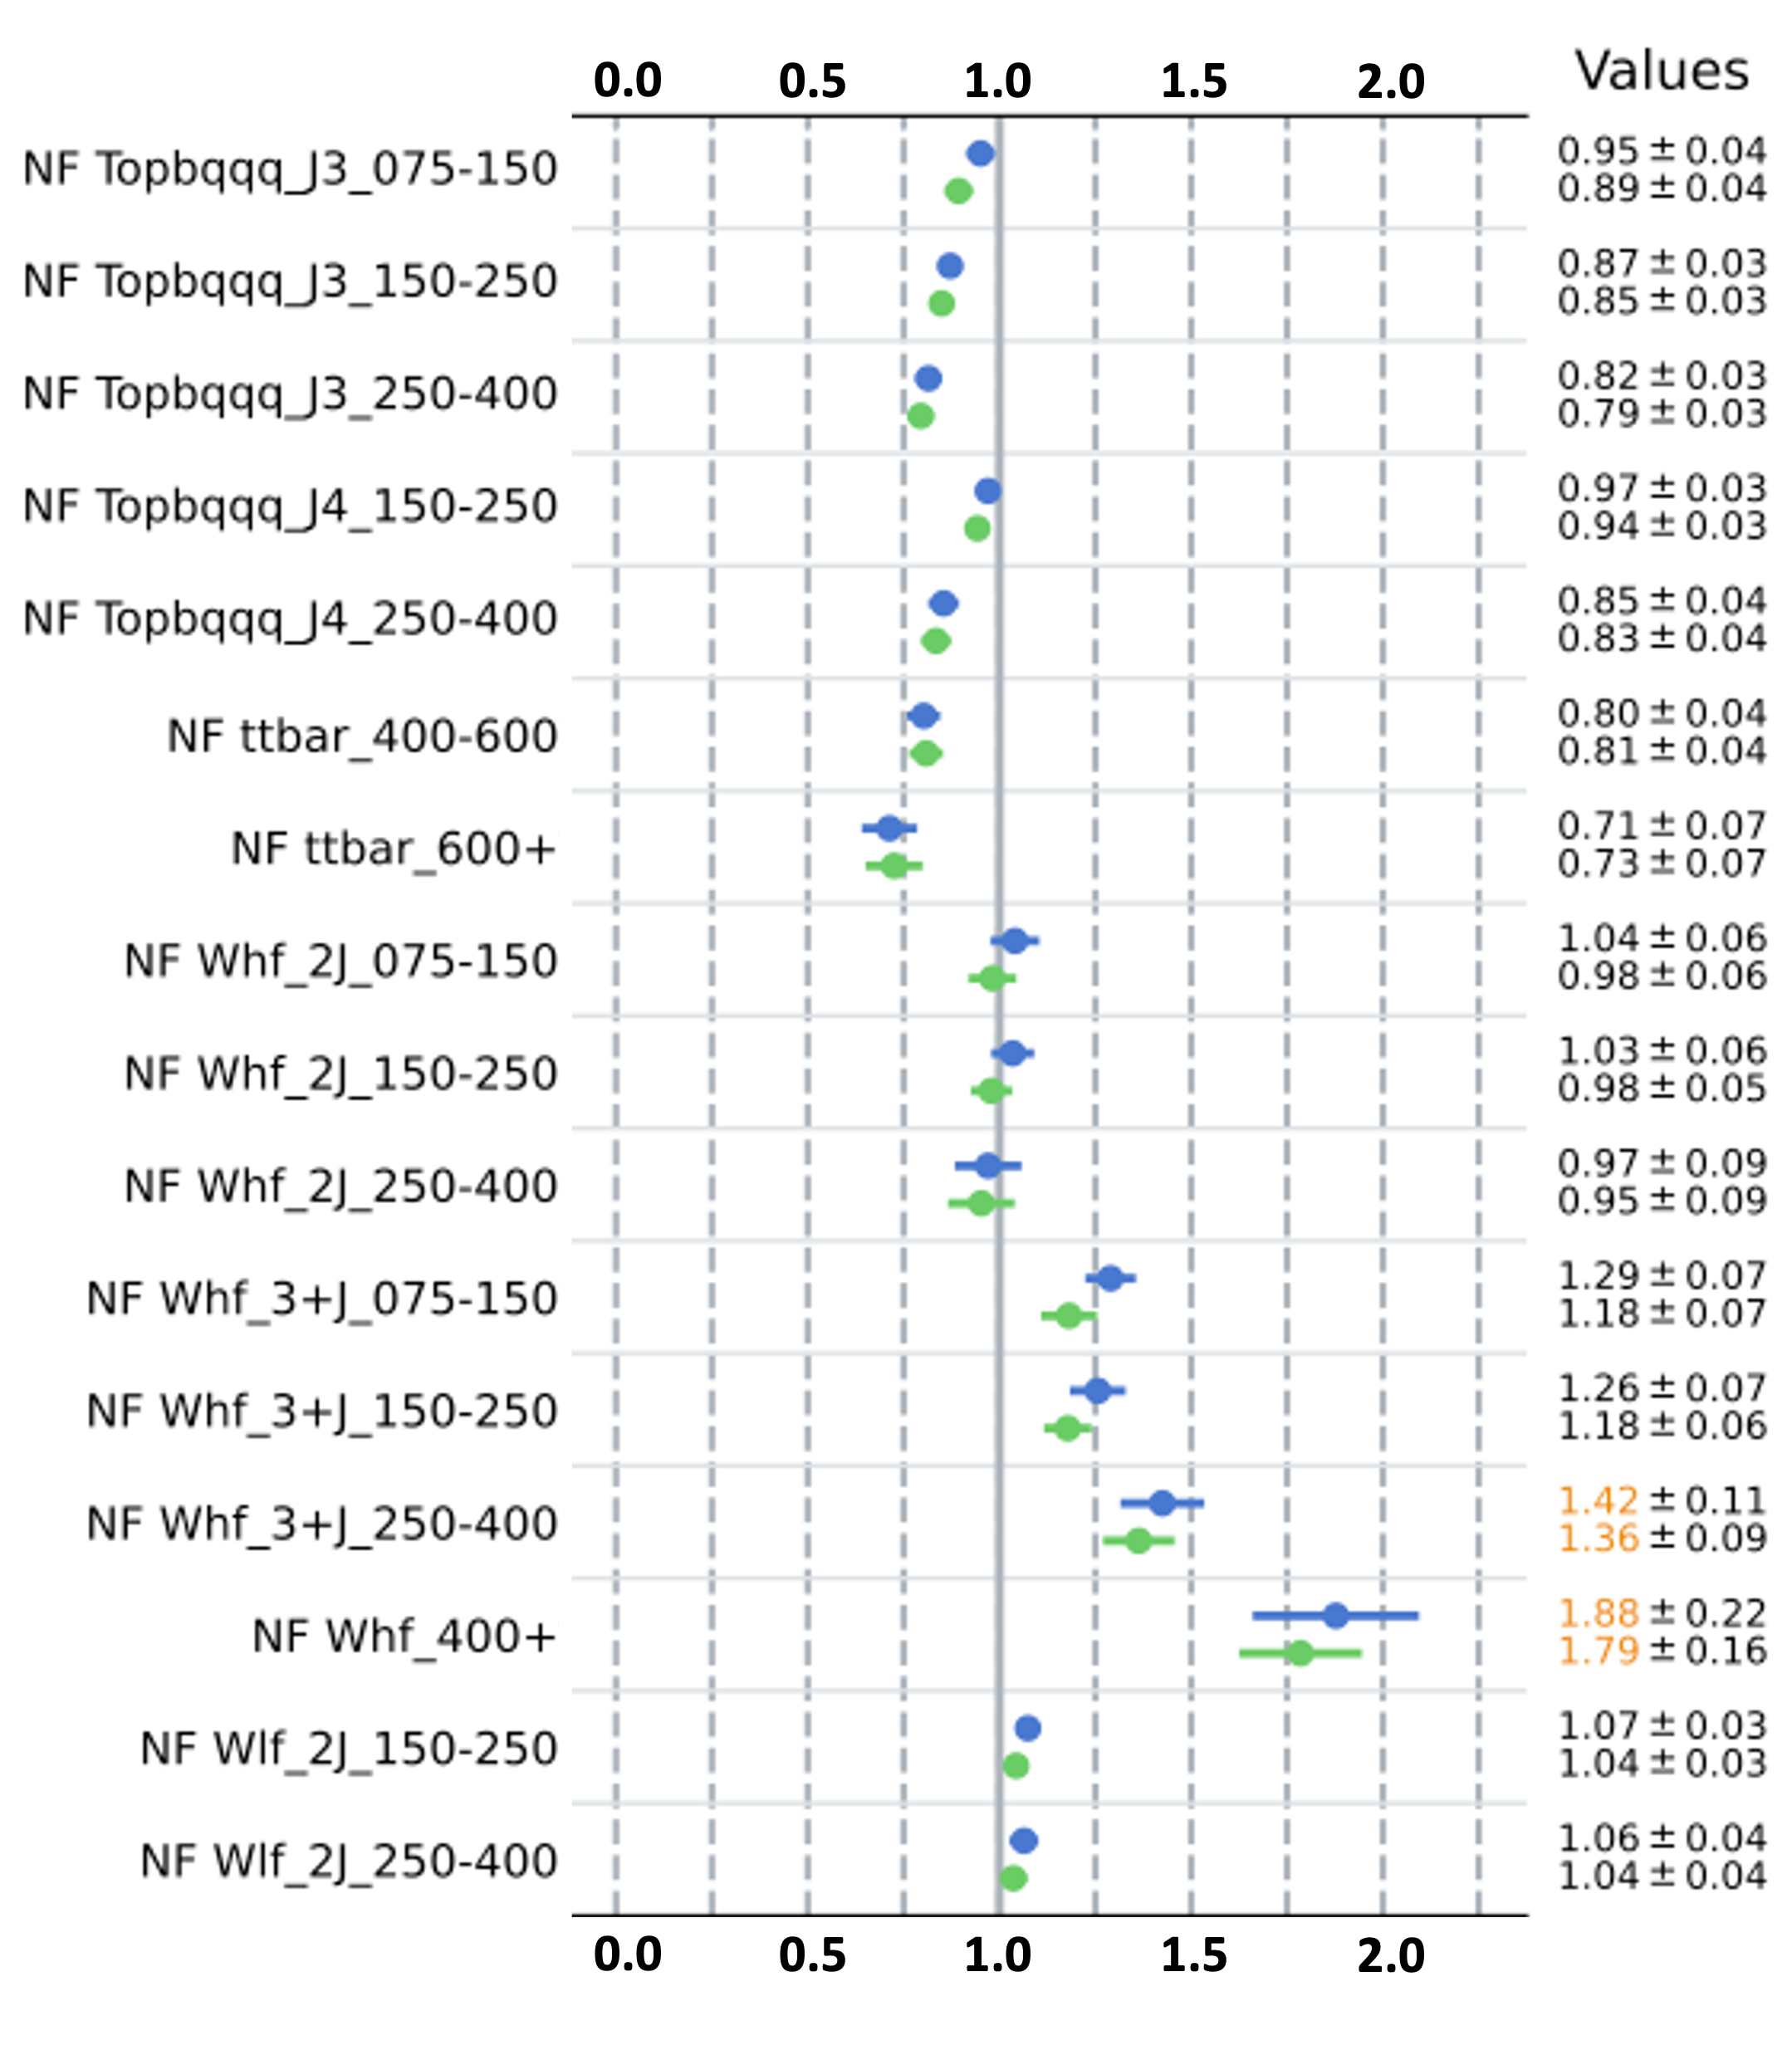
\includegraphics[width=0.49\textwidth]{Images/VH/Fit/fromSlides/FN/FN2.png}\\
    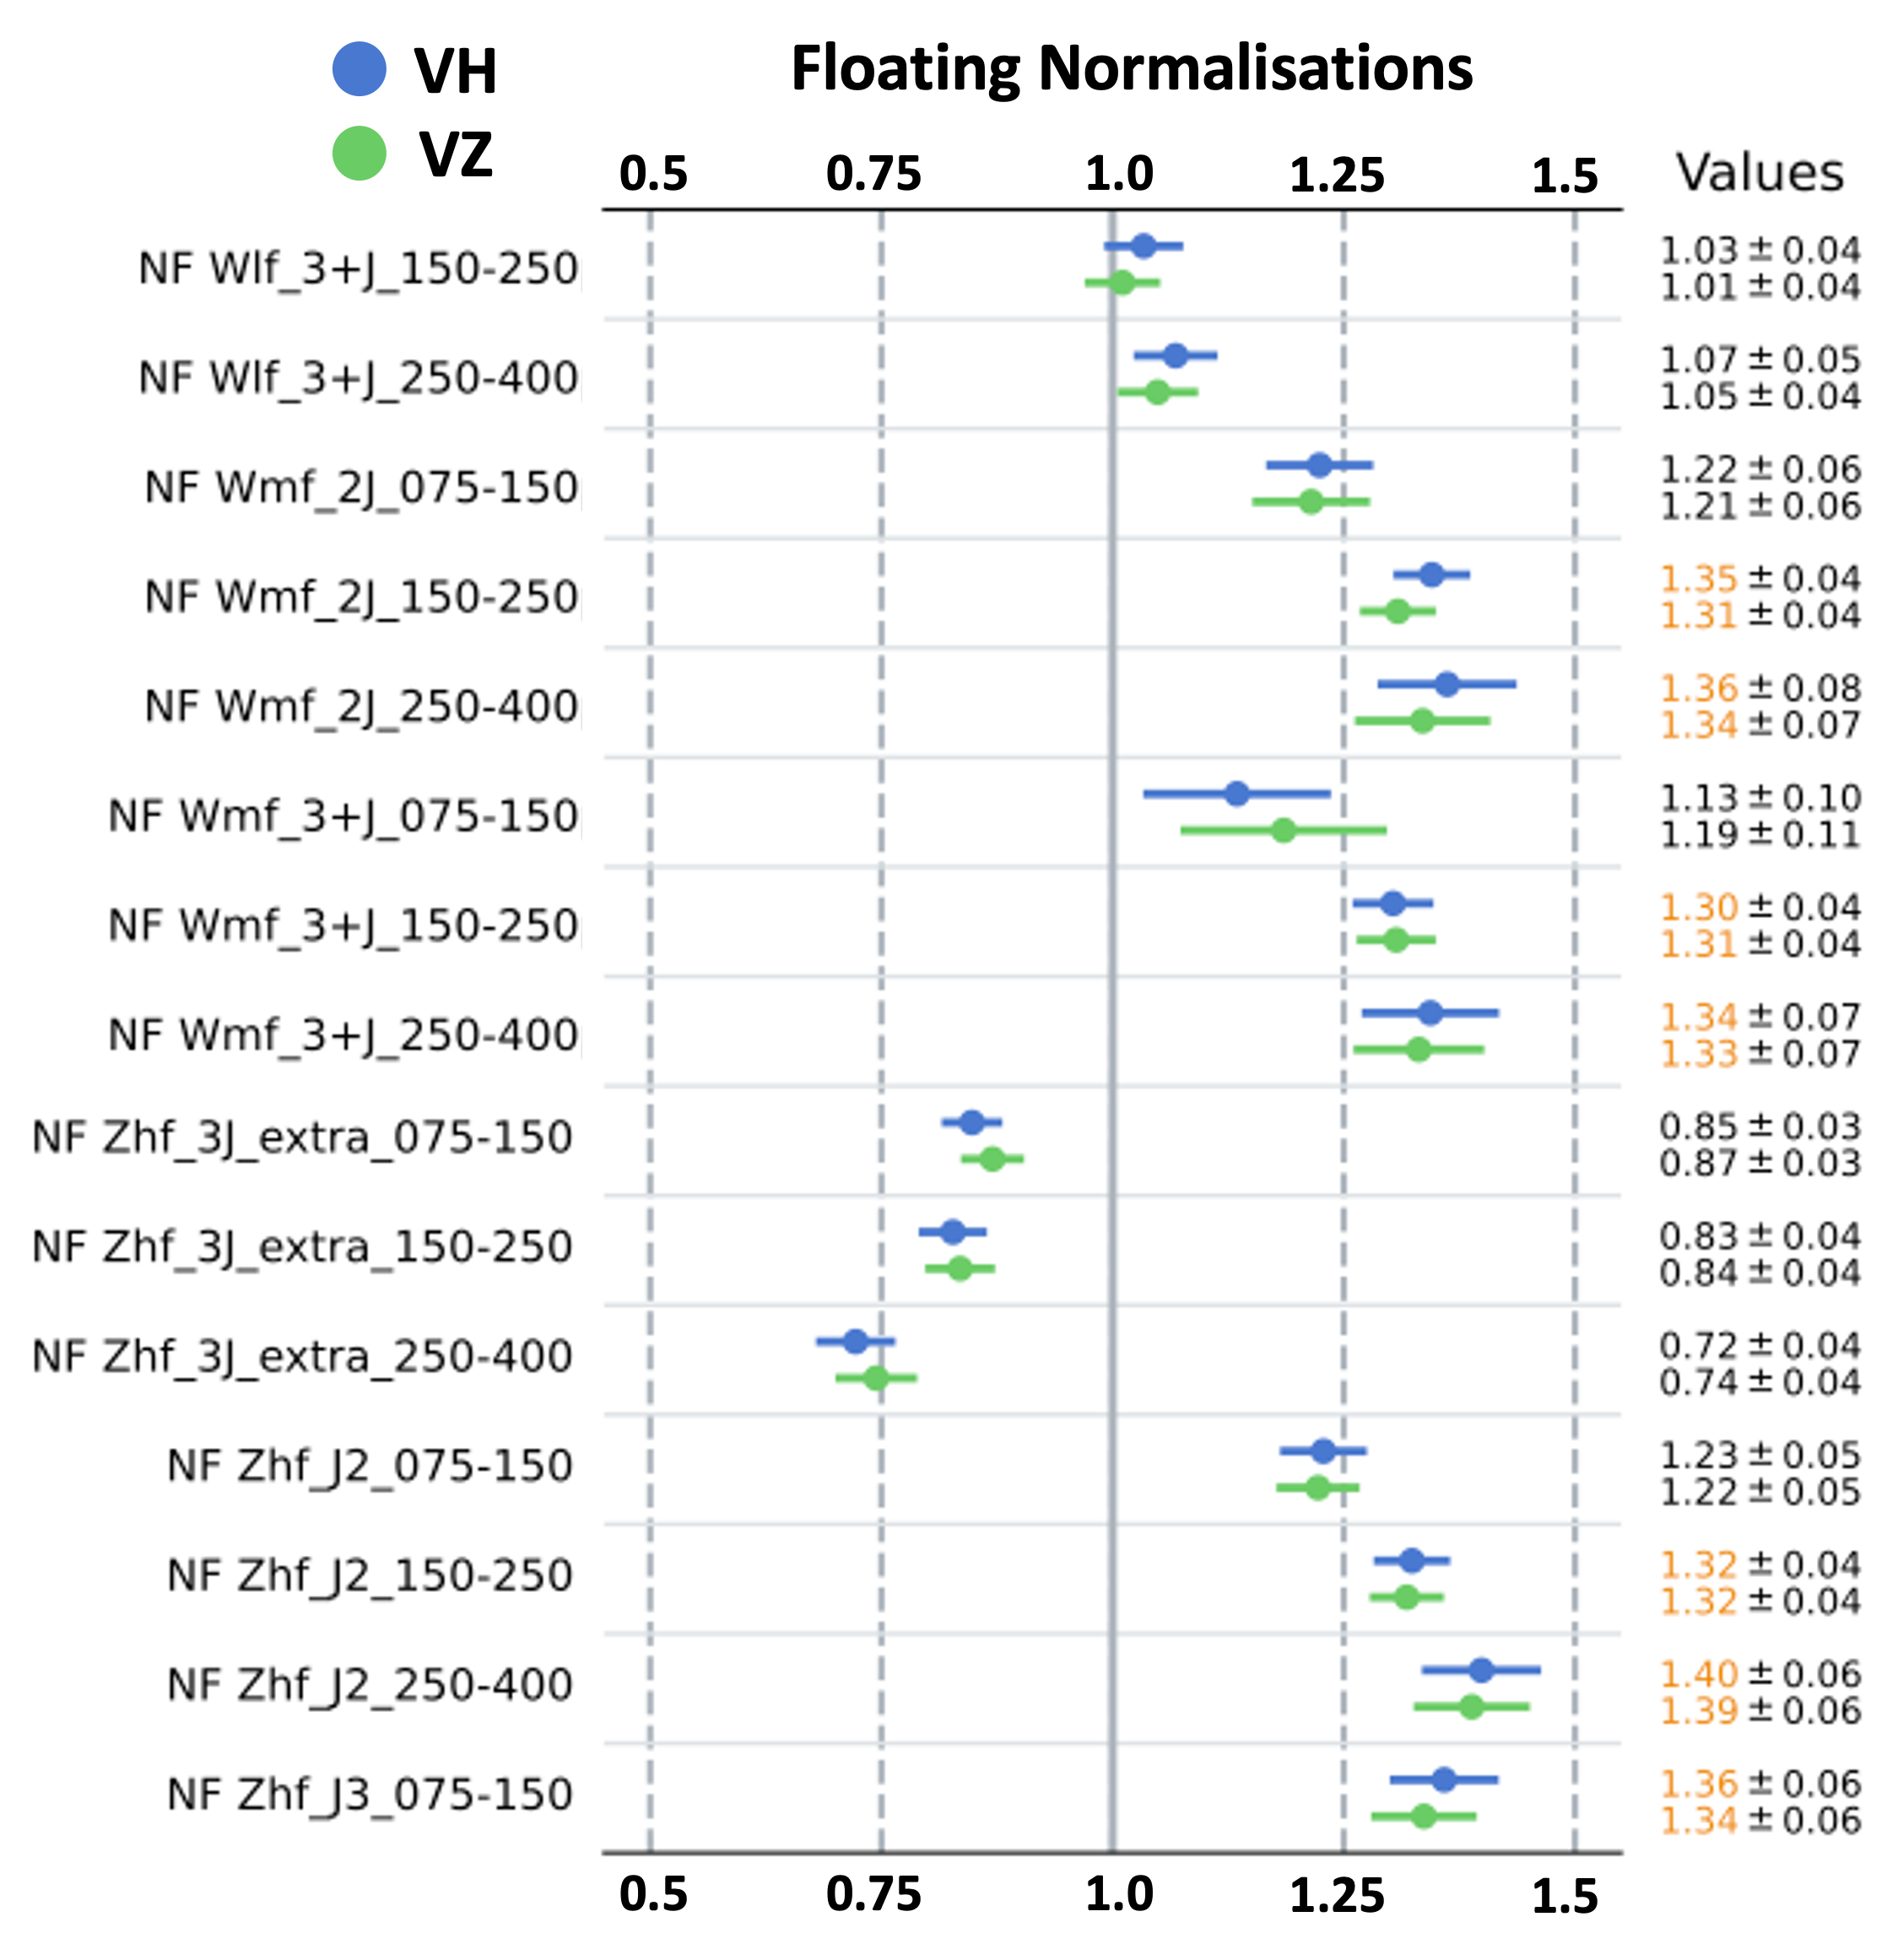
\includegraphics[width=0.49\textwidth]{Images/VH/Fit/fromSlides/FN/FN3.png}
    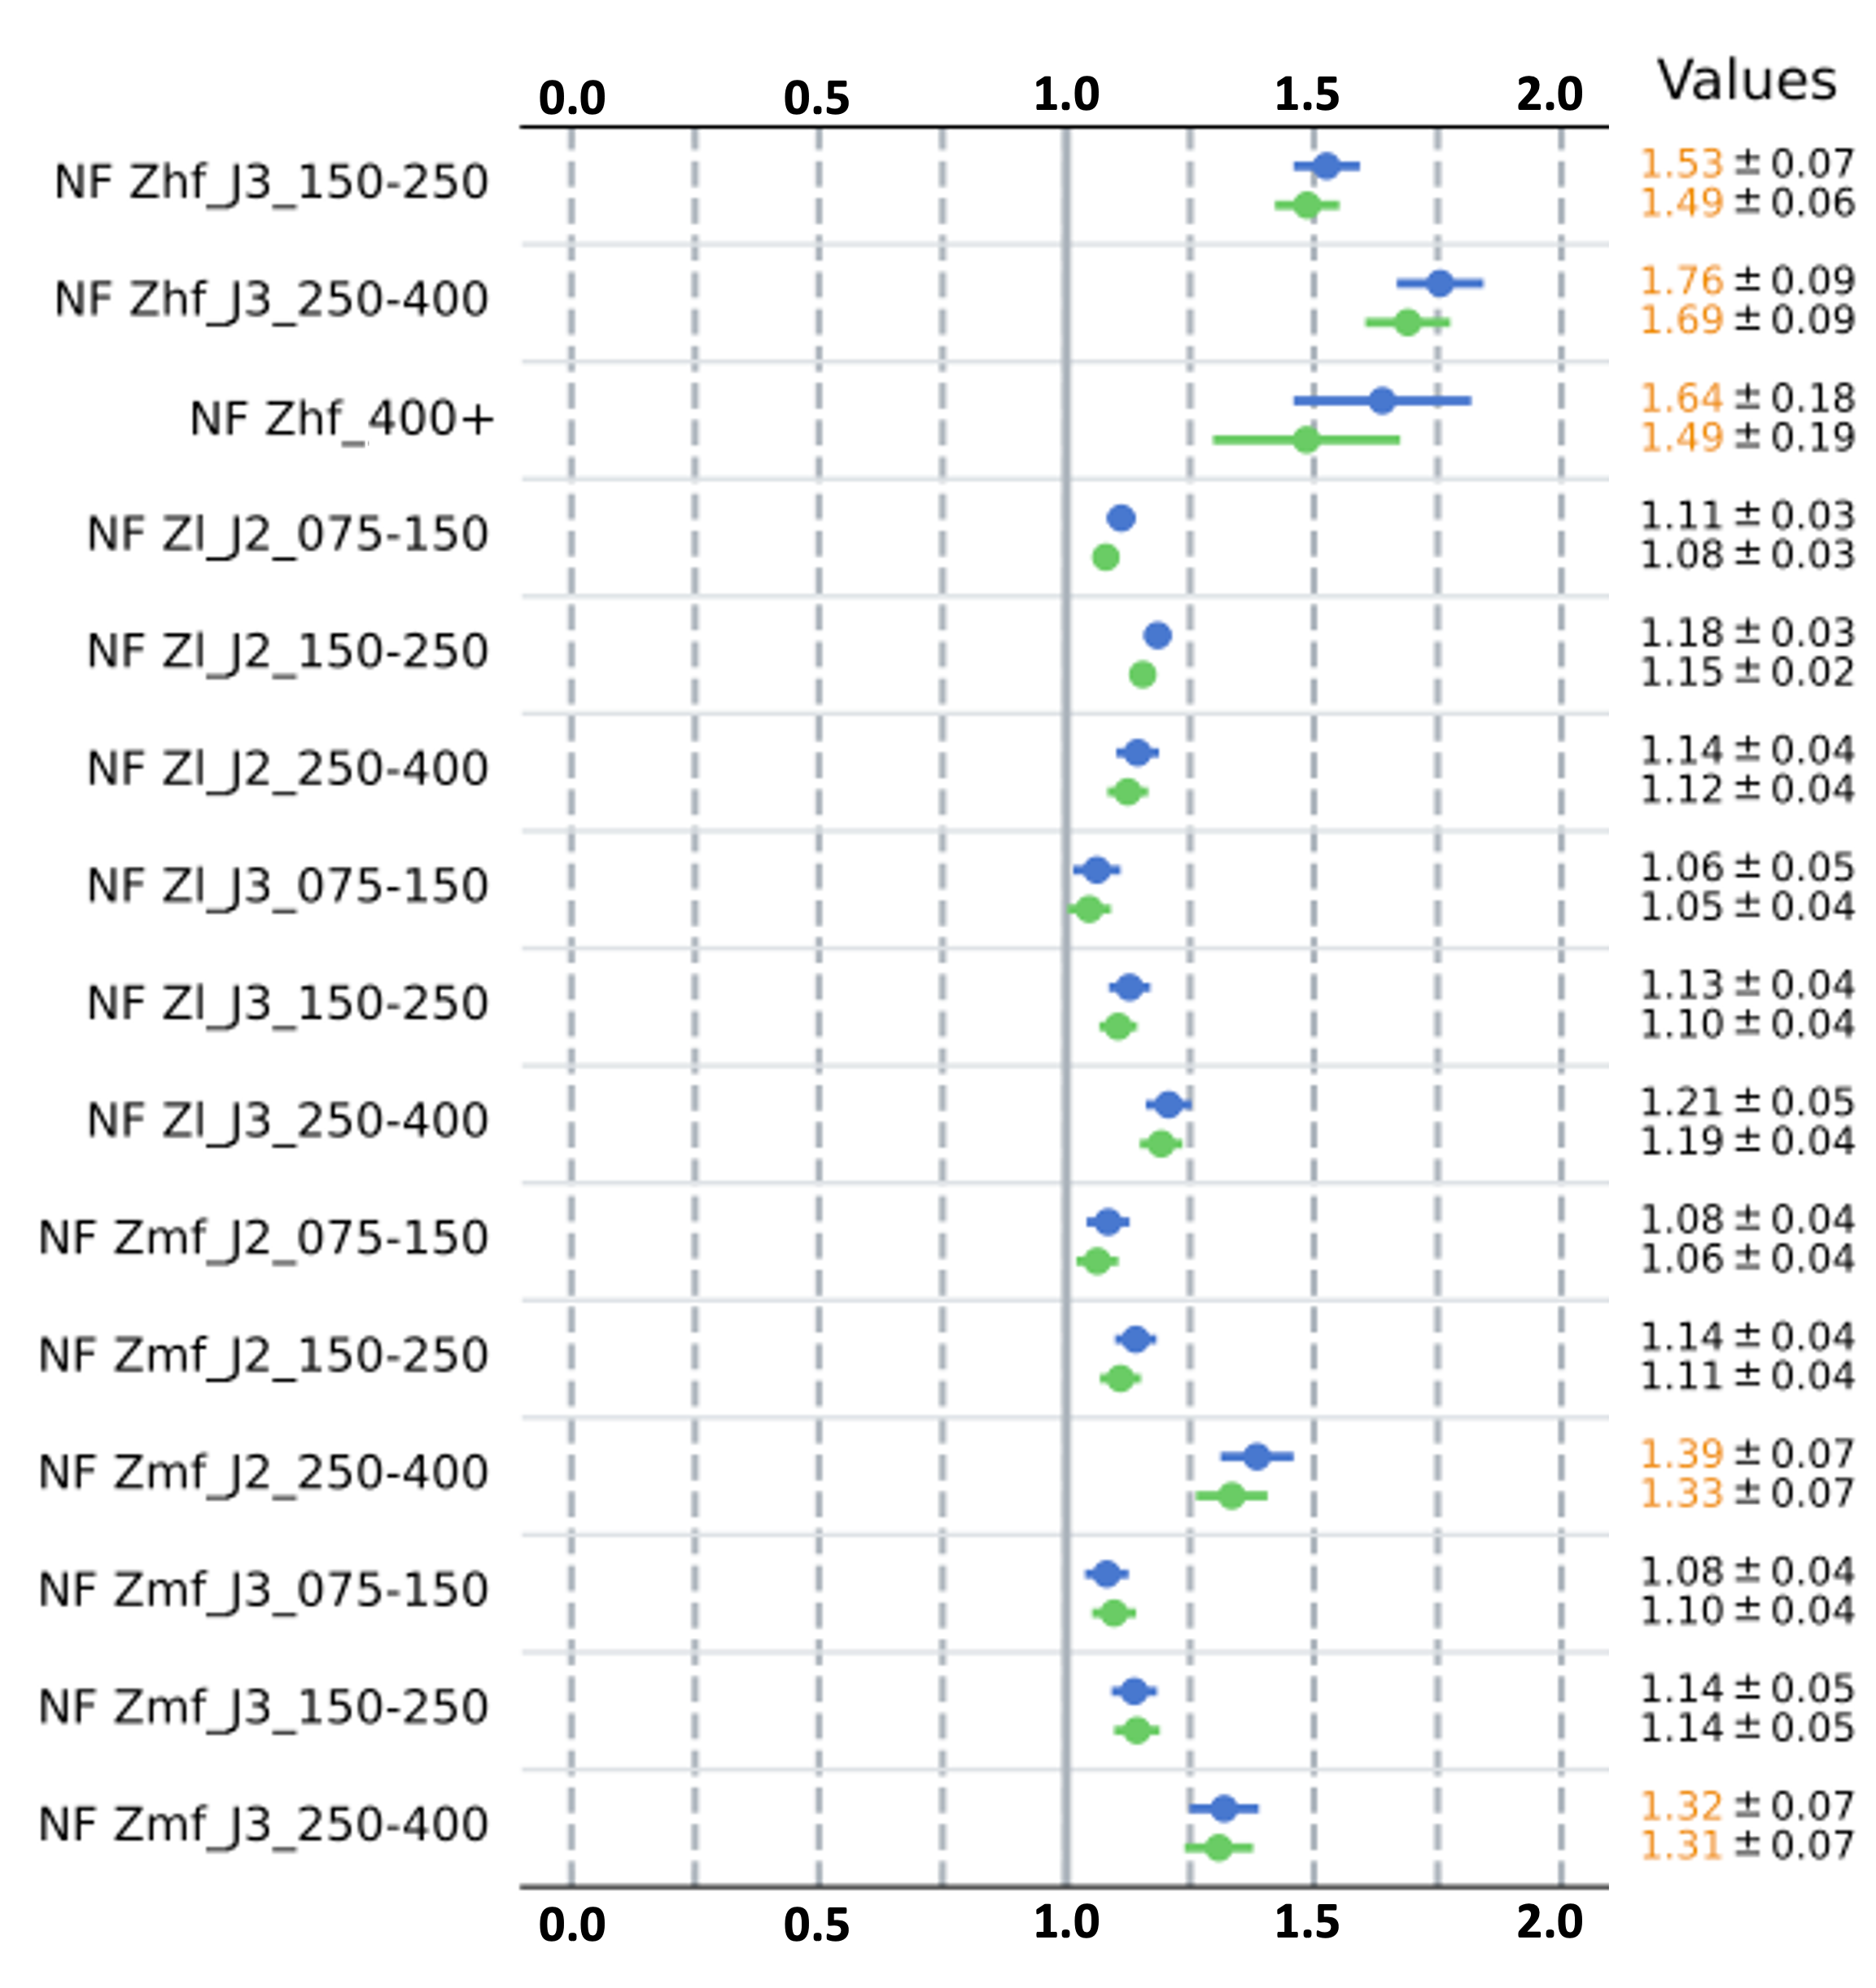
\includegraphics[width=0.49\textwidth]{Images/VH/Fit/fromSlides/FN/FN4.png}
    \caption{The floating normalisations of the major background in the combined analysis targeting the \vhbc\ in blue, versus the cross-check analysis $VZ(\rightarrow b\bar{b}/c\bar{c})$ in green.}
    \label{fig:FNback}
\end{figure} 

\paragraph{}In the combined analysis, the major backgrounds have free-floating normalisations decorrelated across the different \ptv\ and jet multiplicity bins. The values set by a conditional likelihood fit to data, where the \vhbc\ signal strengths are set to their \gls{sm} expectations, are presented in Figure \ref{fig:FNback}. They are compared to the same \glspl{fn} obtained in the cross-check analysis, with $VZ(\rightarrow b\bar{b}/c\bar{c})$ as signals. Good agreement is observed between the two sets of floating normalisations, with some common trends per process highlighted. Concerning the Top backgrounds, in 0L and 1L it seems mostly overestimated in the \gls{mc} simulations, with the overestimation increasing with \ptv. In 2L, the Top process seems well estimated in the Top $e\mu$ \gls{cr}, but the lower statistics available at higher \ptv\ leads to a poor constraining of the floating normalisation. The \glspl{fn} for the Top process are generally better constrained in the 3-jet than the 2-jet category, as expected from the larger yield available for this background at higher jet multiplicities. The Top$(bq/qq)$ and Top$(bb)$ have generally similar \gls{fn} values. Concerning the $W+$jets, the \whf\ is well modelled in 2-jet across \ptv\ but less so in the $\geq$3-jet category, where the underestimation of the simulations grows with \ptv. The boosted \whf\ normalisation in the $\geq$ 400 GeV range is significantly distant higher than unity. The same observations hold for \wlf, which is well-modelled in 2-jet but gets higher \glspl{fn} in 3-jet. The \wmf\ component requires similar large corrections from the fit, with \gls{fn} values $\sim$ 1.3 across the \nj\ and \ptv\ bins. The final background modelled with floating normalisations is $Z+$jets, which also requires significant yield modifications from the fit in all components, jet multiplicity, and \ptv\ bins. The $Z+$jets yield is globally corrected upwards, with larger \gls{fn} values required at higher \ptv. A special case for the \zhf\ is the 3-jet and 3-jet-extra categories, adopted to account for the fact the \vhc\ side does not use 4-jet or separates 3- and $\geq$4-jet in 0L and 2L while the \vhb\ combines 3-jet with 4-jet into $\geq$3-jet in 2L. The 3-jet \glspl{fn} in the figure, labelled ``J3'', cover the $\geq$ 3-jet for \vhb, while the 3-jet-extra, labelled ``3J\_extra'' are only applied to the 3-jet category. There is therefore some overlap, with the latter set of \glspl{fn} used to correct downwards the large normalisation of the $\geq$ 3-jet. Similarly to the \whf, the boosted \zhf\ \gls{fn} values are significantly pulled away from unity.
  
\begin{figure}[h!]
    \hspace{-1.5cm}
    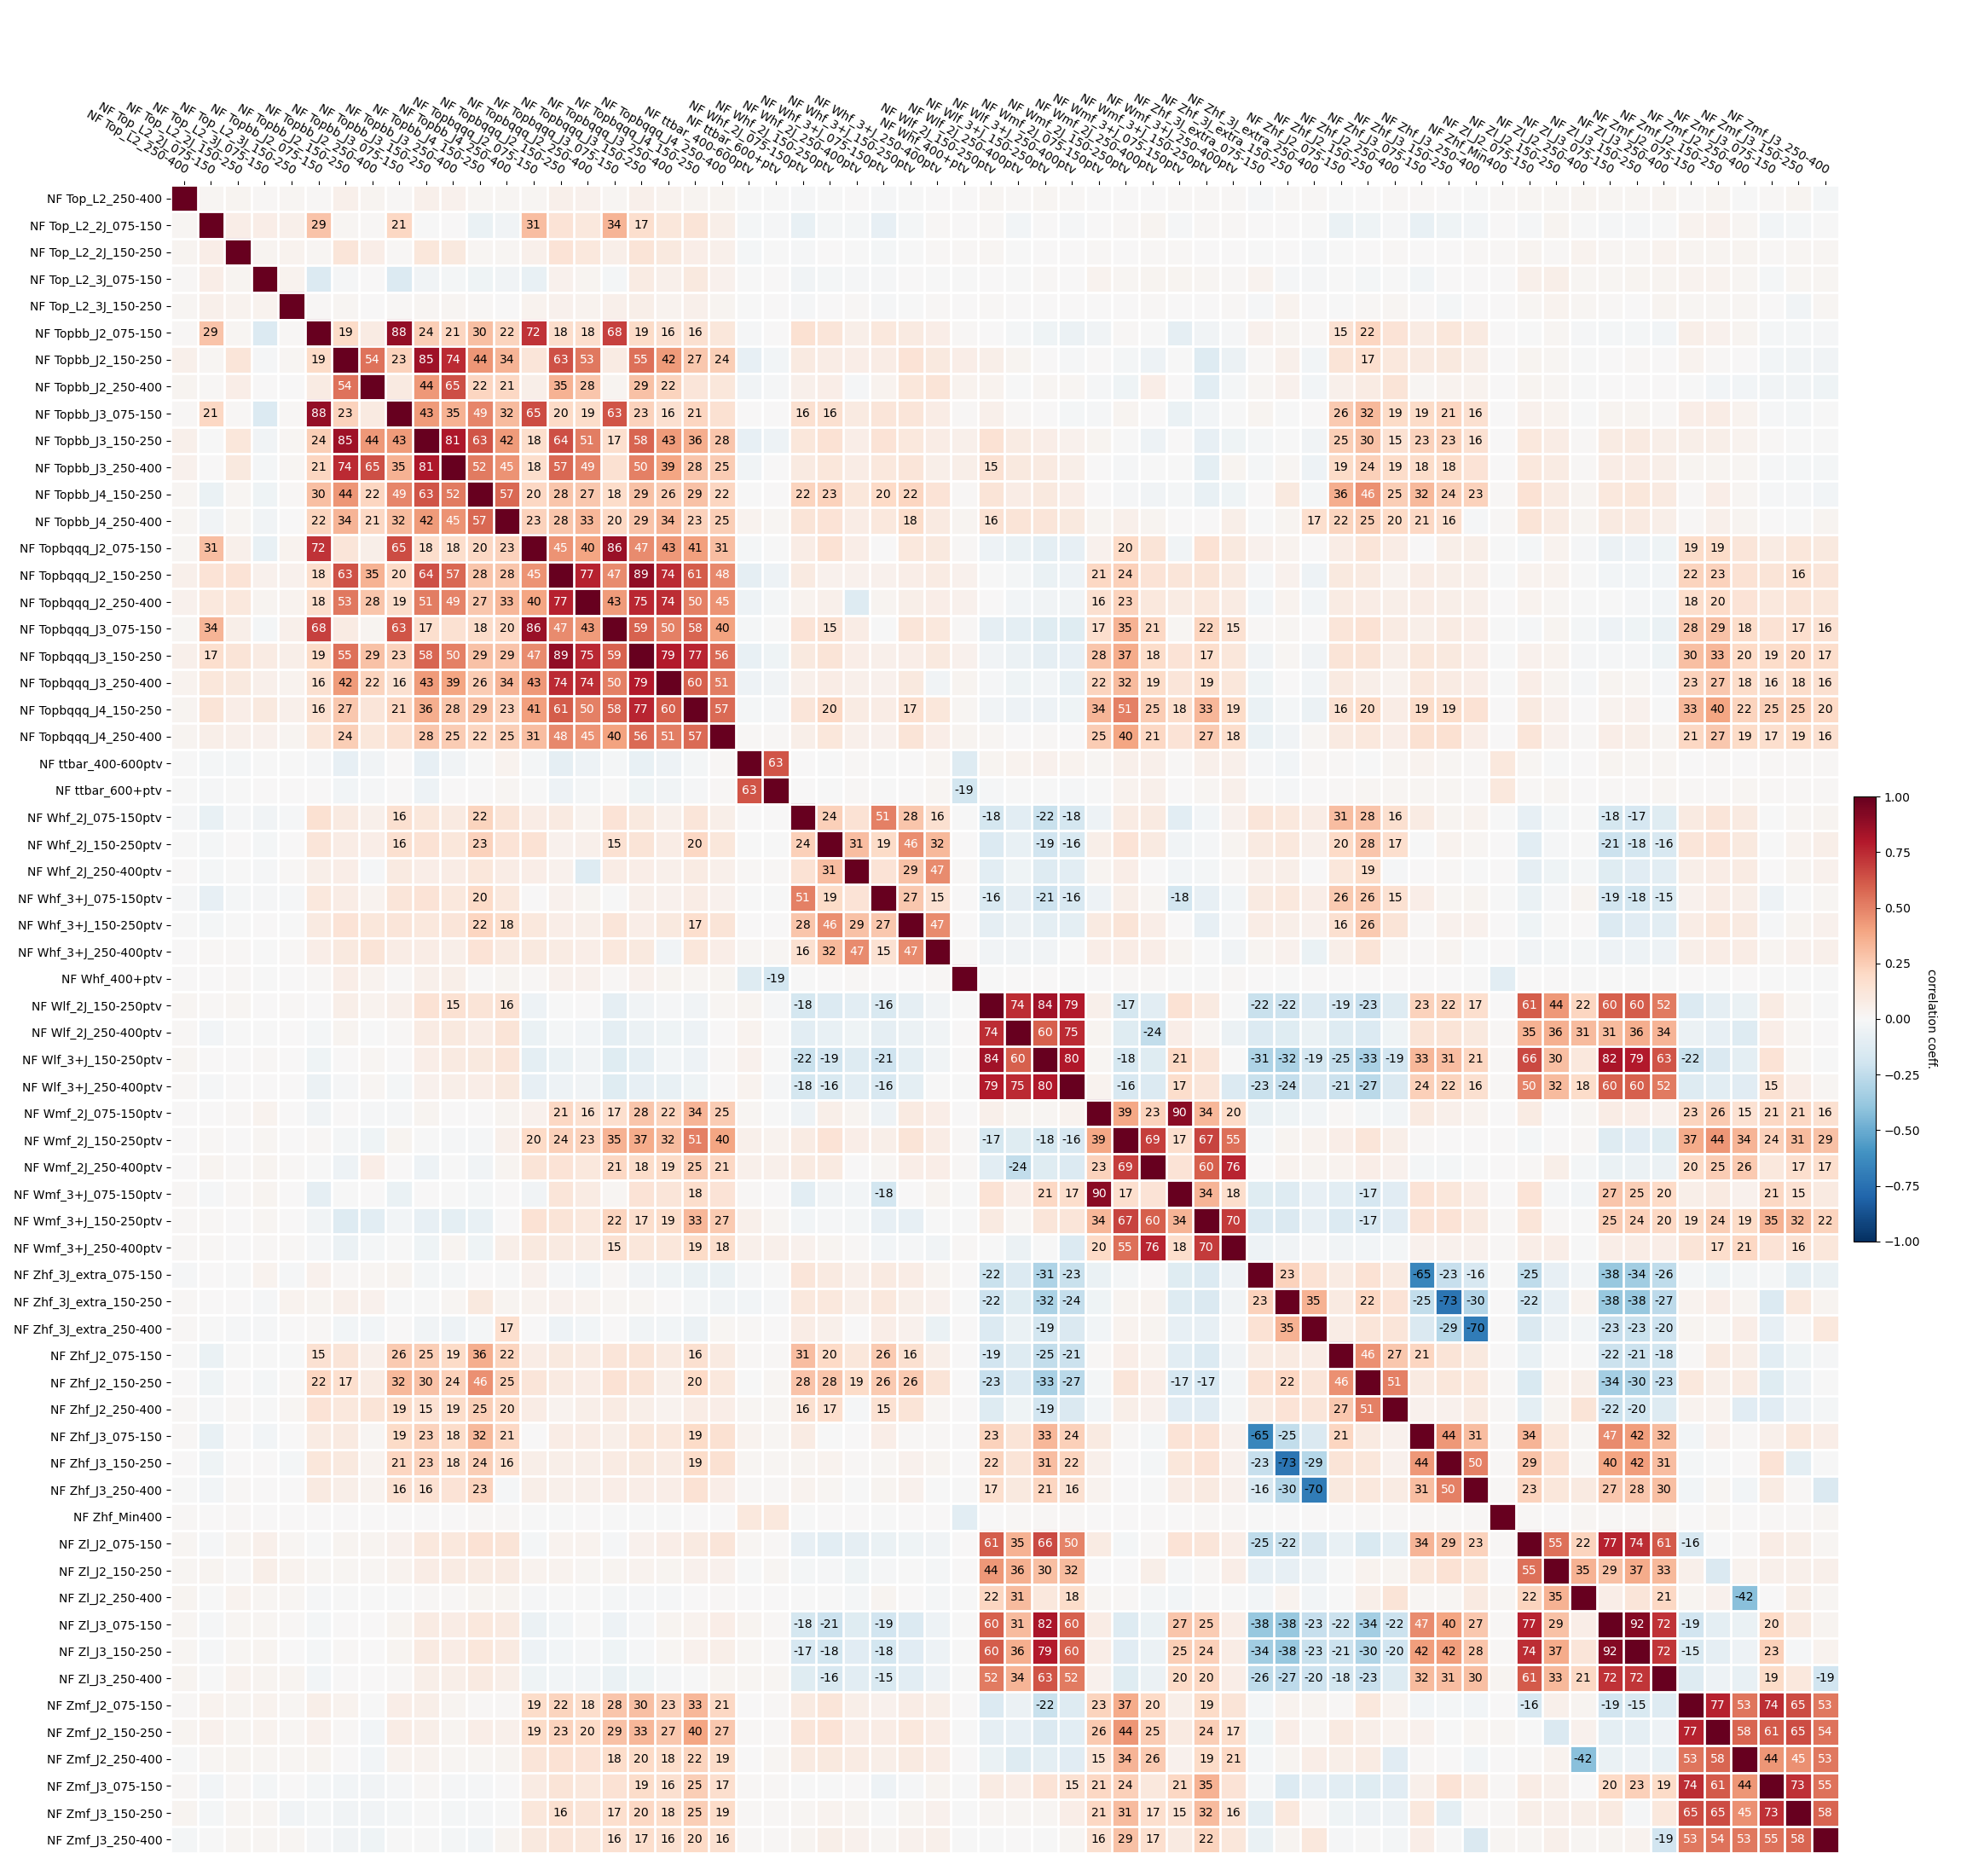
\includegraphics[width=1.15\textwidth]{Images/VH/Fit/fromSlides/SMVHbbcc_2022_MVA_mc16ade_v14.fit_012_fullRes_VHbb_fit_012_012_mc16ade_Systs_mva_VHbbcc_AsimovFit_conditional_mu1_Cov_BTag}
    \caption{The correlations between the floating normalisations of the major background in the combined \vhbc\ analysis.}
    \label{fig:FNcorr}
\end{figure} 

The correlations between the different floating normalisations are displayed as a heat map in Figure \ref{fig:FNcorr}. A rich structure of dependencies emerges from such a plot. As expected, \glspl{fn} related to each process are highly correlated with the other \glspl{fn} of the same process, from different \ptv\ and \nj\ categories. Some striking exceptions are visible: the boosted \ttb\ displays some small uncorrelations with the resolved Top$(bb)$ and Top$(bq/qq)$. Concerning correlations across processes, the Top$(bb)$ and Top$(bq/qq)$ are respectively seen to have large correlations with the \zhf\ (and the \whf\ to a lesser extent) and the \wmf\ and \zmf, as expected from the presence of the $Z+$jets and $W$+jets in the CRHigh and the 0L and 1L Top $BT$ \gls{cr}. The \vhf\ normalisations are slightly anti-correlated to the \vlf, and the \vlf\ are strongly correlated between the $W$ and $Z$.

\section{Conclusion}
This chapter introduces the combined \vhbc\ ATLAS analysis using the 140 fb$^{-1}$ of data collected during Run 2, from 2015 to 2018. The state after its third unblinding approval meeting is presented, as the analysis is not yet concluded. Events are separated based on their \ptv\ into a resolved or boosted regime, as \vhb\ or \vhc\ depending on the two highest tags of their jets or sub-jets. Flavour tagging is performed with the \gls{ml}-based \gls{dl1r} tagger, with a hierarchy of tags ranked as $b$-tagged $>$ tight $c$-tagged $>$ loose $c$-tagged $>$ untagged. This is followed by a split into leptonic channels based on the number of charged lepton $\ell$ ($e$, $\mu$) in the final state, to separate the $Z(\rightarrow \nu\nu)H$, $W(\rightarrow \ell\nu)H$, and $Z(\rightarrow \ell^+\ell^-)H$, with $H \rightarrow b\bar{b}$ or $H \rightarrow c\bar{c}$. To boost the sensitivity, a fine categorisation further splits the analysis space into regions of defined \ptv\ and jet multiplicity. The major backgrounds of the analysis are the $V+$jets and the top processes, the latter grouping the production of \ttb\ pair and the single-top $Wt$. Backgrounds are constrained from data in dedicated control regions, defined respectively by a cut on the angular separation of the Higgs-candidate jets and by an alternative event-tagging selection. The cross-check analysis targeting the $VZ (\rightarrow b\bar{b}/c\bar{c})$ is performed to validate the adopted strategy. \\

The analysis promises to significnatly increase the sensitivity of the ATLAS search for the $H\rightarrow c\bar{c}$ process as well as delivering the finest measurements to date of the differential cross-section of the $H\rightarrow b\bar{b}$. \gls{mva} discriminants are introduced throughout the different regions to improve the sensitivity to the sought signals. The adoption of upgraded flavour tagger and the pseudo-continuous joint-tagging approach paved the way for this coherent joint measurements of the $VH$ to heavy-flavour quarks decay. New \gls{mc} samples with more statistics contribute to reducing the importance of uncertainties plaguing the final fit performance. Some final studies on the modelling strategy and the fit framework are still underway at the time of writing. Some adjustments are required to stabilise the complex fit introduced in this thesis and understand the constrains on the different processes before unblinding the analysis.\\

This study serves as the join combined legacy \vhbc\ analyses of ATLAS on the full Run 2 dataset. Excitingly, progress in the analysis sensitivity to the \vhc\ signal strength has greatly accelerated, with reductions in the upper limit fast approaching the realm of direct measurement of the central value. At the current pace of improvement, the signal strength might be measurable in the next phase of the \gls{lhc}: the High-Luminosity-\gls{lhc} (HL-LHC). Additional improvements to the experimental tools and the analysis strategy are required to reach this threshold. The former will primarily rely on the improved flavour tagging abilities presented in Chapter~\ref{chap-ftag}: from the single tagger \gls{gn2} to the boosted $X \rightarrow b\bar{b} / c\bar{c}$ decay tagger \textit{GN2X} \cite{ATL-PHYS-PUB-2023-021}. The adoption of transformer-based neural networks is promising a significant increase in tagging performance. These will be available for the next iteration of the $VH$ analysis, and is expected to reverberate into an improved signal acceptance and a better background rejection. The larger volume of data to be collected in ongoing Run 3 and following Run 4 of the \gls{lhc} as well as future data-taking campaigns will significantly imrpove the prospects of this severely statistically-limited analysis. 